%% =====================================================================
%% CacheCollapse -- extended journal version
%% Compile with pdfLaTeX + BibTeX (e.g. on Overleaf):
%%   pdflatex main -> bibtex main -> pdflatex main -> pdflatex main
%% The original 2-column conference version is kept as main_v1_conference.tex
%% =====================================================================
\documentclass[preprint,12pt]{elsarticle}

% ---- packages --------------------------------------------------------
\usepackage[T1]{fontenc}
\usepackage[utf8]{inputenc}
\usepackage{lmodern}
\usepackage[margin=1in]{geometry}
\usepackage{amsmath,amssymb,amsfonts}
\usepackage{graphicx}
\usepackage{booktabs}
\usepackage{array}
\usepackage{tabularx}
\usepackage{multirow}
\usepackage{longtable}
\usepackage{textcomp}
\usepackage{xcolor}
\usepackage{url}
\usepackage{caption}
\usepackage{subcaption}
\usepackage{listings}
\usepackage{algorithm}
\usepackage{algpseudocode}
\usepackage{enumitem}
\usepackage{tikz}
\usetikzlibrary{positioning,arrows.meta,shapes.geometric,fit,calc,backgrounds}
\usepackage[hidelinks]{hyperref}

\setlength{\parskip}{3pt}
\renewcommand{\arraystretch}{1.15}
\captionsetup{font=small,labelfont=bf}

% wrapping column types
\newcolumntype{L}[1]{>{\raggedright\arraybackslash}p{#1}}
\newcolumntype{Y}{>{\raggedright\arraybackslash}X}
\newcommand{\yes}{\checkmark}
\newcommand{\no}{$\times$}
\newcommand{\prt}{$\sim$}

% code listings
\definecolor{codebg}{HTML}{F6F6F4}
\definecolor{codekw}{HTML}{1C5CAB}
\definecolor{codecm}{HTML}{6B6A66}
\definecolor{codestr}{HTML}{A8461E}
\lstset{
  basicstyle=\ttfamily\footnotesize,
  backgroundcolor=\color{codebg},
  keywordstyle=\color{codekw}\bfseries,
  commentstyle=\color{codecm}\itshape,
  stringstyle=\color{codestr},
  frame=single, rulecolor=\color{black!20},
  breaklines=true, columns=fullflexible,
  numbers=left, numberstyle=\tiny\color{black!50}, xleftmargin=1.6em,
  showstringspaces=false, captionpos=b
}

\journal{SE-401 Information Security -- Complex Engineering Problem}

\begin{document}

\begin{frontmatter}

\title{CacheCollapse: Reproducing, Detecting, and Mitigating Cache-Stampede-Driven
Indirect Denial of Service in Containerized Web Applications}

\author{Manal Aamir (SE-23070)}
\author{Tayyaba Arshad (SE-23073)}
\author{Noor Afza (SE-23075)}
\author{Batool Fatima (SE-23076)}
\author{Aun Zaidi (SE-23095)}
\address{Department of Software Engineering, NED University of Engineering and
Technology, Karachi, Pakistan}

\begin{abstract}
Containerized web applications almost universally place an in-memory cache between a
stateless application tier and a relational database. This design is efficient under
steady load but hides a structural availability weakness: when a popular cache entry
expires, a burst of otherwise legitimate concurrent requests misses the cache at the
same instant and is forwarded, unthrottled, to the database. The resulting
\emph{cache stampede} converts a modest amount of normal-looking traffic into a flood
of redundant database work. Because the adversary never contacts the database and never
violates an application rule, the event is an \emph{indirect} denial of service that
volume-based network defenses are not designed to catch. This paper presents
\textbf{CacheCollapse}, a fully containerized testbed and defense framework that
(i)~reproduces the cache-stampede attack on a nine-container
Nginx--Flask--Redis--PostgreSQL stack, (ii)~detects it in real time with an
explainable multi-signal rule and an unsupervised IsolationForest trained only on
normal traffic, and (iii)~mitigates it with a layered defense of single-flight cache
locking with stale-while-revalidate, application-layer rate limiting, and edge rate
limiting at the reverse proxy. We analyze 18 monitoring logs (92{,}531 samples,
${\approx}28$~h) and report the final configuration in detail (61{,}923 samples
including 12 undefended attack episodes and 5.6~h of sampled defended attack). Under the undefended attack the median rate of database query attempts rose
from 11 to 108 per second (peak 317), median interval latency from 77 to 174~ms (peak
1{,}159~ms), and 80\% of sampling intervals contained HTTP~503 failures (median
84~failures/s). With the layered defense the median database load fell to
6~queries/s---an 18$\times$ reduction (95\% bootstrap CI 16.8--19.2$\times$)---median
latency fell to 27~ms, and failures were effectively eliminated; recovery after
enabling defenses mid-attack took a median of 1.35~s. The union of the two detectors
caught 12 of 12 attack episodes with one false alarm in 332 normal intervals; the
IsolationForest was fast (median 0.85~s, interval recall 0.91) while the rule was
slower (median 3.2~s, recall 0.27) but perfectly precise and, unlike a volume
threshold that fired on 97\% of absorbed high-volume bursts, never fired on traffic
that the cache absorbed. An ablation and the development history show that cache
locking protects the database but not the proxy path, so edge rate limiting is
required to keep legitimate users fast. We also report measurement caveats uncovered by
the analysis and derive deployment guidance for operators of cached services.
\end{abstract}

\begin{keyword}
Cache stampede \sep thundering herd \sep indirect denial of service \sep
application-layer DDoS \sep containerized security \sep rate limiting \sep cache
locking \sep anomaly detection \sep isolation forest \sep availability
\end{keyword}

\end{frontmatter}

\section*{Highlights}
\begin{itemize}[leftmargin=*]
\item A reproducible nine-container Docker Compose testbed turns an ordinary
Nginx--Flask--Redis--PostgreSQL stack into a controllable cache-stampede laboratory;
an undefended attack drove median database query attempts ${\approx}10\times$ above
baseline (peak ${\approx}29\times$) and produced HTTP~503 failures in 80\% of sampling
intervals.
\item A layered defense (single-flight locking with stale-while-revalidate, application
and edge rate limiting) cut median database load 18$\times$ and median latency
6.4$\times$, held through a 4.5-hour soak under continuous attack, and recovered in a
median of 1.35~s when enabled mid-attack.
\item Across 12 attack episodes, a multi-signal rule (precision 1.00) and an
unsupervised IsolationForest (recall 0.91) jointly detected every attack; the rule
never fired on high-volume traffic that the cache absorbed, whereas a volume threshold
fired on 97\% of it.
\item Analysis of the logs exposes non-obvious measurement pitfalls---the cache-miss
rate is a weak stampede signal under short TTLs, and goodput collapses to
${\approx}23$ completed queries/s, far below nominal pool capacity---and yields concrete
deployment guidance.
\end{itemize}

\clearpage
\tableofcontents
\clearpage

%% =====================================================================
\section{Introduction}
\label{sec:intro}
%% =====================================================================

The availability of a web service is as much a security property as its
confidentiality or integrity. Denial-of-service (DoS) attacks remain among the most
common and most damaging threats to online systems, and the research community has
produced extensive taxonomies and defenses for network- and transport-layer flooding
\cite{mirkovic2004,zargar2013}. Large botnets such as Mirai have shown that raw
volumetric capacity is cheap for an adversary to obtain \cite{antonakakis2017}. A
harder class of attacks, however, operates at the application layer: the adversary
issues syntactically and semantically valid requests that are individually
indistinguishable from those of legitimate users, so that volume- or signature-based
filters are ineffective or must be tuned so aggressively that they harm real customers
\cite{praseed2019,xie2009,ranjan2009}. This paper studies a particularly subtle member
of that class in the setting in which most modern software is now deployed: the
containerized, multi-service web application.

\subsection{Motivation: the Cache as an Attack Surface}
Virtually every read-heavy web application interposes an in-memory cache such as
Redis or memcached between its application tier and its database, so that repeated
requests for the same object are answered from memory rather than recomputed
\cite{fitzpatrick2004,nishtala2013}. Each cached entry receives a time-to-live (TTL),
after which it expires and must be regenerated from the database. The cache is usually
discussed as a \emph{performance} component, but it also changes the \emph{capacity
model} of the system: once a cache is in place the database is typically provisioned
only for the residual miss traffic, not for the full request rate. Production
workloads are highly skewed towards a small set of popular (``hot'') keys
\cite{breslau1999,atikoglu2012}, so the protection the cache provides is concentrated
on exactly those keys.

If a hot key expires while many requests for it are in flight, all of them miss the
cache at the same instant and are forwarded to the database simultaneously. A single
expiry therefore produces not one query but $N$ redundant queries, where $N$ is the
instantaneous concurrency on that key. This is a \emph{cache stampede}, also called a
\emph{dog-pile} or \emph{thundering herd}, and it is documented as a first-order hazard
in large-scale systems \cite{vattani2015,nishtala2013}. The consequences can be
severe even without an adversary: Facebook's widely discussed outage of September 2010
was attributed to an automated system that, on seeing an invalid cached configuration
value, caused every client to query the backing database cluster at once, overwhelming
it in a self-reinforcing loop \cite{johnson2010}. Practitioner guidance on cascading
failure likewise identifies the loss of a cache layer as one of the classic triggers of
system-wide overload \cite{beyer2016}.

What is less often treated is that the same mechanism is a \emph{security}
vulnerability. An adversary who understands a target's caching behavior can
deliberately align bursts of requests for hot objects with those objects' expiry,
repeatedly, so that the database is driven into overload by traffic that never leaves
the normal request distribution of the application. The database---not the web
server---is the victim, and the web application is merely the conduit. We call this
an \emph{Indirect Distributed Denial of Service} (IDDoS): \emph{indirect} because the
attacker never addresses the victim component, and \emph{distributed} in its effect
because the damage is produced by the fan-out of concurrency inside the system rather
than by the attacker's own request volume. Because the attack rides on correct
application logic rather than on a software defect, it cannot be ``patched''; it must
be \emph{detected} and \emph{mitigated} as an operational property of the system, in
the same way that algorithmic-complexity attacks exploit legitimate but expensive code
paths \cite{crosby2003} and low-rate attacks exploit legitimate protocol timers
\cite{kuzmanovic2003}.

\subsection{Problem Statement and the Complex Engineering Challenge}
Defending this vulnerability in a containerized environment is a genuine complex
engineering problem: its difficulty arises from the \emph{interaction} of
well-understood components rather than from any single exotic one. Three tensions
must be resolved simultaneously.

\begin{enumerate}[label=\textbf{T\arabic*.},leftmargin=*]
\item \textbf{Detection without a volumetric signature.} The attack's request rate at
the web tier can resemble a legitimate spike or flash crowd \cite{jung2002,kandula2005}.
A detector keyed on request volume alone will either miss the attack or raise
constant false alarms on benign bursts that the cache absorbs harmlessly.
\item \textbf{Mitigation without self-inflicted denial of service.} A defense that
simply rejects traffic to protect the database can itself become the denial of
service. The mitigation must shed the \emph{redundant} load while continuing to serve
genuine users quickly.
\item \textbf{Faithful, safe, repeatable experimentation.} Studying an availability
attack requires driving a realistic system into failure repeatedly and measuring
per-component behavior, which demands an isolated, resettable, production-like
environment rather than a single-process simulation---and one that cannot harm any
third party.
\end{enumerate}

These requirements are coupled. An overly aggressive guardrail degrades legitimate
users; a cache-only fix that ignores the connection path leaves users slow even when
the database is healthy (Section~\ref{sec:ablation}); and a detector that is evaluated
only on the traffic it was tuned on can look perfect while measuring the wrong thing
(Section~\ref{sec:det-results}). Resolving the problem therefore requires an integrated
architectural, algorithmic, and experimental design, not merely a faster database or a
larger cache.

\subsection{Research Questions}
The work is organized around four research questions:
\begin{description}[leftmargin=1.2em,style=nextline]
\item[RQ1 (Reproduction).] Can a cache-stampede IDDoS be reproduced deterministically
on an ordinary containerized stack using only well-formed requests, and what are its
quantitative effects on database load, latency, and availability?
\item[RQ2 (Mechanism).] Which mechanism converts the stampede into user-visible failure,
and can its magnitude be predicted from simple system parameters (key count, TTL,
request rate, connection-pool size)?
\item[RQ3 (Detection).] How do an explainable multi-signal rule and an unsupervised
IsolationForest compare in detection latency, coverage, false alarms, and
interpretability---and how do they compare with naive single-signal detectors?
\item[RQ4 (Mitigation).] Which combination of cache locking, stale-while-revalidate,
and rate limiting restores availability, how quickly, and what does each layer
contribute?
\end{description}

\subsection{Proposed Solution}
We present \textbf{CacheCollapse}, a framework that addresses all three tensions
together:
(i)~a \emph{reproducible containerized testbed} that reconstructs the
Nginx~$\rightarrow$~Flask~$\rightarrow$~Redis~$\rightarrow$~PostgreSQL request path on
an isolated Docker Compose network \cite{merkel2014,dockercompose} and generates both
normal traffic and a controllable stampede attack;
(ii)~a \emph{dual detection subsystem} pairing an explainable multi-signal rule with
an unsupervised IsolationForest \cite{liu2008,liu2012} trained only on baseline
behavior; and
(iii)~a \emph{layered mitigation} combining single-flight cache locking with
stale-while-revalidate \cite{nishtala2013,rfc5861}, an application-layer per-client
rate limiter, and an edge rate limiter at the reverse proxy \cite{nginxlimitreq}, each
of which can be toggled live from a browser dashboard while the attack is running.

\subsection{Contributions}
\begin{itemize}[leftmargin=*]
\item A \textbf{containerized IDDoS testbed} that reproduces the cache-stampede attack
on nine interacting industry-standard services, with a Redis-based control plane that
switches traffic, attack, and each defense on and off live
(Section~\ref{sec:design}).
\item An \textbf{analytical model} of baseline miss traffic, stampede amplification,
and defended load that predicts the measured baseline database rate to within 9\%
and explains why, under overload, completed database work collapses far below
nominal pool capacity (Sections~\ref{sec:model} and~\ref{sec:mechanics}).
\item A \textbf{multi-signal rule-based detector} and an \textbf{unsupervised
IsolationForest detector}, and a detailed comparison on 12 attack episodes and
${\approx}1{,}100$ labelled intervals covering detection latency, interval-level
precision and recall, behavior on idle and defended traffic, threshold sensitivity,
ROC analysis, and training-window sensitivity (Section~\ref{sec:det-results}).
\item A \textbf{layered mitigation}, an \textbf{ablation}, and a \textbf{longitudinal
analysis} of 14 experiment sessions showing how each engineering fix changed
defended-mode latency and request admission, including the deployment-critical
finding that database-level and proxy-level protection are distinct and both
required (Sections~\ref{sec:mitigation-results}--\ref{sec:ablation}).
\item A \textbf{fully reproducible, instrumented deployment} (single
\texttt{docker compose up}, Prometheus/Grafana, live dashboard, demonstration
storefront) validated by a 16-case automated end-to-end test suite, plus an explicit
account of \textbf{measurement pitfalls} in the instrumentation that other
practitioners are likely to repeat (Section~\ref{sec:validity}).
\end{itemize}

\subsection{Paper Organization}
Section~\ref{sec:background} reviews the technical background on caching, overload,
rate limiting, and anomaly detection. Section~\ref{sec:related} surveys related work
and identifies the research gap. Section~\ref{sec:threat} defines the threat model and
develops an analytical model of the attack. Section~\ref{sec:design} describes the
design and implementation of CacheCollapse. Section~\ref{sec:method} sets out the
experimental methodology and dataset. Section~\ref{sec:results} presents the results
for each research question. Section~\ref{sec:comparative} compares CacheCollapse with
prior work and alternative mitigations. Section~\ref{sec:discussion} discusses
implications, engineering lessons, threats to validity, and limitations, and
Section~\ref{sec:conclusion} concludes. Appendices give a reproduction guide, key
configuration listings, and a mapping of the project to the attributes of a complex
engineering problem.

%% =====================================================================
\section{Background}
\label{sec:background}
%% =====================================================================

This section introduces the concepts on which the rest of the paper depends: caching
patterns and expiry semantics, the cache stampede, overload behavior of connection
pools, rate-limiting algorithms, unsupervised anomaly detection with isolation
forests, and the container and observability tooling used by the testbed.

\subsection{Caching Patterns and Expiry Semantics}
\label{sec:bg-caching}
Three caching patterns dominate web back ends \cite{kleppmann2017}:
\begin{itemize}[leftmargin=*]
\item \textbf{Cache-aside (lazy loading).} The application reads the cache; on a miss
it reads the database and writes the result into the cache. The cache never talks to
the database itself. This is the pattern used by CacheCollapse and by the memcache
deployment described by Nishtala et al.\ \cite{nishtala2013}.
\item \textbf{Read-through.} The cache library itself loads missing values from the
database, which centralizes regeneration but does not by itself prevent concurrent
regeneration of the same key.
\item \textbf{Write-through / write-behind.} Writes update the cache and the database
together (or asynchronously), keeping entries fresh and reducing reliance on expiry.
\end{itemize}
Expiry is usually governed by a TTL. Short TTLs bound staleness but increase the
rate of expiries; long TTLs reduce database load but serve older data. HTTP caching
formalizes a useful middle ground: the \texttt{stale-while-revalidate} directive
allows a cache to serve a stale response for a bounded period while it refreshes the
entry in the background \cite{rfc5861}. CacheCollapse applies the same idea inside
the application tier.

Popularity in real workloads is strongly skewed; web object requests follow a
Zipf-like distribution \cite{breslau1999}, and large key--value workloads concentrate
a large fraction of requests on a small set of keys \cite{atikoglu2012}. Skew is what
makes caching effective, and also what makes a few hot keys a single point of
failure: Fan et al.\ show that a small front-end cache is needed precisely to prevent
hot keys from overloading individual back-end nodes \cite{fan2011}.

\subsection{The Cache Stampede}
\label{sec:bg-stampede}
Consider a hot key $k$ with TTL $T$ and regeneration time $d$ (the time to compute the
value from the database). Let requests for $k$ arrive at rate $\lambda_k$. If the
entry expires at time $t_{\mathrm{exp}}$, every request arriving in
$(t_{\mathrm{exp}}, t_{\mathrm{exp}}+d)$ finds the cache empty. In a naive cache-aside
implementation each of those requests independently regenerates the value, so the
expected number of database queries caused by one expiry is
\begin{equation}
\mathbb{E}[Q_{\mathrm{exp}}] \approx 1 + \lambda_k d ,
\label{eq:stampede}
\end{equation}
and for a synchronized burst of $B$ concurrent requests it is simply $B$. Equation
\eqref{eq:stampede} has two important properties. First, the redundant work grows
with $d$, and $d$ itself grows as the database becomes loaded---a positive feedback
loop. Second, it is \emph{independent of the TTL}; a longer TTL makes stampedes less
frequent but not smaller.

Four families of mitigation exist:
(i)~\emph{request coalescing} (single-flight), in which only one caller regenerates a
key and the others wait for or reuse its result \cite{nishtala2013,singleflight};
(ii)~\emph{serving stale data} during regeneration \cite{rfc5861,nygard2018};
(iii)~\emph{early or probabilistic recomputation} before expiry, which Vattani et al.\
show can be made optimal with the XFetch rule \cite{vattani2015}; and
(iv)~\emph{TTL jitter}, which de-synchronizes expiries of keys that were filled at the
same time. Only the first two remove redundancy once a synchronized burst has already
arrived; the latter two reduce the probability that it happens.

\subsection{Connection Pools, Queueing, and Overload}
\label{sec:bg-queueing}
An application reaches its database through a bounded pool of $c$ connections. If each
query holds a connection for $d$ seconds, the pool's nominal service capacity is
\begin{equation}
\mu_{\max} = \frac{c}{d}\quad\text{queries/s.}
\label{eq:capacity}
\end{equation}
Little's law, $L=\lambda W$ \cite{little1961}, relates the mean number of in-flight
requests $L$ to the arrival rate $\lambda$ and mean residence time $W$; as $\lambda$
approaches $\mu_{\max}$ the residence time---and thus latency---grows without bound in
classical queueing models \cite{kleinrock1975}. Pools differ in what happens at
saturation. A \emph{blocking} pool queues callers, converting overload into latency;
a \emph{fail-fast} pool rejects them, converting overload into errors. The psycopg2
\texttt{ThreadedConnectionPool} used here is fail-fast: requesting a connection from
an exhausted pool raises an exception immediately \cite{psycopgpool}.

A well-known pathology of overloaded systems is that useful throughput (\emph{goodput})
can \emph{fall} as offered load rises, because more and more work is spent on requests
that will ultimately be rejected or time out. This is the essence of congestion
collapse in networks \cite{jacobson1988} and of receive livelock in operating systems
\cite{mogul1997}. Overload-control research therefore argues for shedding excess load
\emph{early}, at the edge of the system, before it consumes scarce resources
\cite{welsh2001,welsh2003,cherkasova2002,beyer2016}. Tail latency compounds the
problem: in fan-out services, a small fraction of slow components dominates
user-perceived latency \cite{dean2013}.

\subsection{Rate-Limiting Algorithms}
\label{sec:bg-ratelimit}
Rate limiting caps the rate at which a client (or a class of clients) may consume a
resource. Table~\ref{tab:ratelimit-algos} summarizes the algorithms relevant to this
work. The \emph{leaky bucket} smooths output to a constant rate and is the basis of
Nginx's \texttt{limit\_req} module \cite{nginxlimitreq,tanenbaum2011}; a configurable
burst allowance lets short spikes through without delay (\texttt{nodelay}). A
\emph{fixed-window counter} is the simplest to implement on a shared store such as
Redis: a counter keyed by client and time window is incremented on each request and
compared with a threshold. Rate limiting can be enforced locally or across a cluster
\cite{raghavan2007}. HTTP defines status 429 (Too Many Requests) for requests rejected
by a rate limiter \cite{rfc6585}, distinguishing intentional shedding from server
failure (status 503).

\begin{table}[t]
\centering
\caption{Rate-limiting algorithms relevant to CacheCollapse.}
\label{tab:ratelimit-algos}
\small
\begin{tabularx}{\linewidth}{@{}L{2.6cm}YYL{2.6cm}@{}}
\toprule
Algorithm & Mechanism & Strengths / weaknesses & Used here \\
\midrule
Fixed window & Counter per client per window; reject above limit & Trivial on Redis; allows up to $2\times$ limit across a window boundary & Flask app layer (1~s window, 50 req/s) \\
Sliding window & Weighted counts over the last window & Smoother than fixed window; more state & -- \\
Token bucket & Tokens accrue at rate $r$ up to depth $b$; a request spends one & Permits bursts up to $b$; average rate $r$ & -- \\
Leaky bucket & Requests drain from a queue at constant rate $r$ & Smooth output; with \texttt{burst}/\texttt{nodelay} behaves like a token bucket & Nginx edge (\texttt{limit\_req}, 50 r/s, burst 20) \\
Admission control & Admit/reject by measured load & Adapts to capacity; needs a load signal & Discussed (Sec.~\ref{sec:discussion}) \\
\bottomrule
\end{tabularx}
\end{table}

\subsection{Anomaly Detection and the Isolation Forest}
\label{sec:bg-iforest}
Intrusion detection has long been split between \emph{misuse} (signature or rule)
detection and \emph{anomaly} detection, which models normal behavior and flags
deviations \cite{denning1987}. Anomaly detection is attractive for attacks without a
fixed signature, but it is notoriously sensitive to the base rate of attacks
\cite{axelsson2000}, and machine-learning detectors that perform well in the
laboratory often fail operationally because ``anomalous'' is not the same as
``malicious'' \cite{sommer2010}. Surveys organize outlier detection by technique and
by the availability of labels \cite{chandola2009,hodge2004}.

The \emph{Isolation Forest} (iForest) \cite{liu2008,liu2012} is an unsupervised
ensemble method that isolates anomalies directly rather than profiling normal points.
Each of $t$ trees is grown on a sub-sample of $\psi$ points by repeatedly choosing a
random feature and a random split value between that feature's minimum and maximum,
until each point is isolated or a height limit is reached. Anomalies, being few and
different, are isolated near the root, so their path length $h(x)$ is short. The
anomaly score of a point $x$ is
\begin{equation}
s(x,\psi) = 2^{-\frac{\mathbb{E}[h(x)]}{c(\psi)}}, \qquad
c(\psi) = 2H(\psi-1) - \frac{2(\psi-1)}{\psi},
\label{eq:iforest}
\end{equation}
where $\mathbb{E}[h(x)]$ is the mean path length over the trees, $H(i)\approx\ln i +
0.5772$ is the harmonic number, and $c(\psi)$ normalizes by the average path length of
an unsuccessful binary-search-tree lookup. Scores near 1 indicate anomalies; scores
well below 0.5 indicate normal points. The scikit-learn implementation
\cite{pedregosa2011} exposes a \texttt{decision\_function} (positive for inliers,
negative for outliers) whose threshold is set by a \texttt{contamination} parameter,
the expected fraction of outliers in the training data. Isolation forests require no
labels, train in near-linear time, and work well with small samples, which makes them
suitable for learning a ``normal'' profile from a few seconds of live traffic. Unlike
the supervised random forests from which they borrow the ensemble idea
\cite{breiman2001}, they cannot learn what an attack looks like---only what normal
looks like.

\subsection{Containers and Observability}
\label{sec:bg-containers}
Containers package an application with its dependencies and isolate it using kernel
namespaces and control groups \cite{merkel2014,pahl2015}; orchestrators from Docker
Compose \cite{dockercompose} to Kubernetes \cite{burns2016} wire many containers into
a microservice application \cite{dragoni2017}. Containers bring their own security
concerns, chiefly around isolation and configuration \cite{combe2016,sultan2019}, but
for this study their key property is \emph{reproducibility}: an entire multi-service
system can be created, attacked, measured, and destroyed from a single declarative
file. Observability is provided by Prometheus, a pull-based time-series system that
periodically scrapes text-format metrics endpoints \cite{brazil2018}, visualized with
Grafana. For low-latency browser dashboards, Server-Sent Events (SSE) provide a simple
one-way push channel over HTTP.

%% =====================================================================
\section{Literature Review}
\label{sec:related}
%% =====================================================================

We organize prior work into six threads: cache stampedes and large-scale caching;
denial of service and application-layer attacks; attacks that target caching
infrastructure; availability attacks in cloud and container environments; overload
control; and detection. We close with a literature matrix and the research gap.

\subsection{Cache Stampede and the Thundering Herd}
Fitzpatrick's description of memcached established the cache-aside pattern that most
web systems still follow \cite{fitzpatrick2004}. Nishtala et al., describing
Facebook's memcache deployment, identify ``stale sets'' and ``thundering herds'' as
first-order concerns and introduce \emph{leases}: a per-key token that permits only
one client to regenerate a missing value while others briefly wait or accept slightly
stale data. They report that leases substantially reduce peak database query rates
\cite{nishtala2013}. Vattani, Chierichetti, and Lowenstein formalize the mitigation
side and derive an optimal \emph{probabilistic early recomputation} rule (XFetch) in
which an item is refreshed before its TTL with a probability that rises as expiry
approaches \cite{vattani2015}. Workload studies of large key--value stores
\cite{atikoglu2012} and of photo caching at scale \cite{huang2013} confirm the
heavy skew that makes hot-key protection critical, and Fan et al.\ show that a small
cache in front of a partitioned service provably balances load only if it holds the
hottest keys \cite{fan2011}.

All of these works treat the stampede as a \emph{performance} hazard arising from
benign load. CacheCollapse builds directly on their mitigation insights---single-flight
regeneration is the descendant of memcache leases---but reframes the stampede as an
\emph{attacker-triggerable} availability vulnerability, adds detection, and measures
end-to-end user-visible availability rather than database load alone.

\subsection{Denial of Service and Application-Layer Attacks}
Classical DDoS research classifies attacks and defenses mainly at the network and
transport layers. Mirkovic and Reiher give the canonical taxonomy of attacks and
defenses \cite{mirkovic2004}, and Zargar et al.\ survey flooding defenses, stressing
that protection must span prevention, detection, and response \cite{zargar2013}.
Application-layer DoS is distinct and harder. Xie and Yu model normal browsing behavior
to detect attacks composed of ordinary HTTP GET requests \cite{xie2009}; Ranjan et al.\
propose DDoS-Shield, which assigns suspicion scores to sessions and schedules requests
to limit the damage of attackers mimicking legitimate clients \cite{ranjan2009};
and Praseed and Thilagam survey the space, emphasizing that such attacks can be
mounted at low volume with legitimate requests \cite{praseed2019}.

A central difficulty is distinguishing attacks from \emph{flash crowds}---sudden,
legitimate surges of interest. Jung et al.\ characterize flash crowds and DoS attacks
and propose distinguishing features such as client distribution and per-client request
rates \cite{jung2002}; Kandula et al.\ address attacks that deliberately mimic flash
crowds by using CAPTCHAs and admission control to separate humans from bots
\cite{kandula2005}. Two further lines show that damaging attacks need not be
voluminous: low-rate ``shrew'' attacks exploit TCP's retransmission timer with
carefully timed bursts \cite{kuzmanovic2003}, and algorithmic-complexity attacks feed
inputs that trigger the worst-case behavior of legitimate data structures
\cite{crosby2003}. The cache-stampede IDDoS shares the timing element of the former and
the ``legitimate but expensive path'' element of the latter: requests are legitimate,
the aggregate web-tier rate need not be anomalous, and the damage is produced
downstream by cache semantics.

\subsection{Attacks that Target Caching Infrastructure}
A growing body of work treats caches themselves as attack surfaces. Triukose et al.\
show that content-delivery networks can be abused to amplify load on an origin server
by requesting uncacheable or cache-busting URLs \cite{triukose2009}. Guo et al.\
demonstrate that CDN forwarding behavior can be turned against the very origin it is
meant to protect (``CDN Judo'') \cite{guo2020}. Nguyen et al.\ introduce
\emph{cache-poisoned denial of service} (CPDoS), in which an attacker causes an
intermediate HTTP cache to store an error page that is then served to every subsequent
user \cite{nguyen2019}. These works share our view that caching changes the threat
model, but they target shared HTTP caches at the network edge and the integrity of
cached content. CacheCollapse targets the \emph{application-internal} cache and the
database behind it, and its attack requires neither cache-busting parameters nor
poisoned content---only correct timing.

\subsection{Availability Attacks in Cloud and Containerized Environments}
Containers are the dominant packaging and orchestration unit for modern applications
\cite{pahl2015,merkel2014,burns2016}, and the microservice style decomposes
applications into many interacting services \cite{dragoni2017}. Security analyses of
Docker catalog isolation and configuration weaknesses \cite{combe2016,sultan2019}, but
availability has received comparatively less attention. The most directly relevant
line is the \emph{Yo-Yo attack}, in which periodic bursts drive an auto-scaling
controller to oscillate between scale-up and scale-down, degrading performance and
inflating cost while evading simple volume detection \cite{sides2016,bremlerbarr2017}.
CacheCollapse is complementary: like Yo-Yo it exploits an emergent property of a
cloud-native pattern (there, elasticity; here, caching) using legitimate-looking
traffic, and like Yo-Yo it must be studied in an orchestrated, resettable environment.
Unlike Yo-Yo, it causes damage without any auto-scaler and in a single deployment.

\subsection{Overload Control and Graceful Degradation}
Systems research has long argued that services should degrade gracefully under
overload. SEDA structures a server as stages connected by queues with admission
controllers so that overload is shed explicitly \cite{welsh2001}, and Welsh and Culler
later propose adaptive overload control driven by measured response times
\cite{welsh2003}. Session-based admission control rejects new sessions under load to
preserve service for sessions already in progress \cite{cherkasova2002}. Practitioner
literature codifies related stability patterns---timeouts, circuit breakers, bulkheads,
and serving stale data---\cite{nygard2018}, and site-reliability practice treats load
shedding, client throttling, and protection against cache loss as defenses against
cascading failure \cite{beyer2016}. Rate limiting may be enforced at a single proxy or
globally across replicas \cite{raghavan2007}. A contribution of the present paper is to
show empirically that these controls are \emph{not} interchangeable in the stampede
setting: coalescing protects the database, edge rate limiting protects the request
path, and only their combination preserves end-to-end availability.

\subsection{Detection: Rules, Statistics, and Machine Learning}
Denning's intrusion-detection model introduced statistical profiles of normal behavior
as a basis for detecting attacks \cite{denning1987}. Chandola et al.\ and Hodge and
Austin survey anomaly detection broadly, underlining that the choice of method
depends on label availability, data type, and interpretability requirements
\cite{chandola2009,hodge2004}. Two cautionary results shape our evaluation. Axelsson
shows that because attacks are rare, even a small false-positive rate can make most
alarms false \cite{axelsson2000}; and Sommer and Paxson argue that machine-learning
detectors face a ``closed world'' problem in which anything not seen in training is
flagged, so that operational benign changes look like attacks \cite{sommer2010}. Among
unsupervised methods the Isolation Forest \cite{liu2008,liu2012} is widely used because
it needs no labels and few samples. We therefore pair it with an explainable rule and
evaluate both not only on attack and normal traffic but also on idle and defended
traffic, where the closed-world problem becomes visible. ROC analysis \cite{fawcett2006}
is used to separate the ranking quality of a score from the choice of threshold.

\subsection{Literature Matrix and Research Gap}
Table~\ref{tab:litmatrix} summarizes the most relevant works, what they contribute, and
what they leave open relative to the problem studied here.

\begin{table}[p]
\centering
\caption{Literature matrix: focus, approach, and gap relative to CacheCollapse.}
\label{tab:litmatrix}
\footnotesize
\begin{tabularx}{\linewidth}{@{}L{2.7cm}L{2.6cm}YY@{}}
\toprule
Work & Focus & Approach / key finding & Gap relative to this paper \\
\midrule
Nishtala et al.\ 2013 \cite{nishtala2013} & Caching at scale & Leases coalesce regeneration; stale sets & Performance framing; no adversary, no detection \\
Vattani et al.\ 2015 \cite{vattani2015} & Stampede prevention & Optimal probabilistic early recomputation (XFetch) & Assumes benign load; does not handle a burst that is already in flight \\
Fan et al.\ 2011 \cite{fan2011} & Load balancing & Small front cache balances partitioned back ends & Capacity planning, not attack/defense \\
Mirkovic \& Reiher 2004 \cite{mirkovic2004} & DDoS taxonomy & Classifies attacks and defenses & Network-layer focus \\
Zargar et al.\ 2013 \cite{zargar2013} & DDoS defense survey & Prevention--detection--response framing & Flooding attacks; no cache semantics \\
Xie \& Yu 2009 \cite{xie2009} & App-layer DDoS detection & Models normal browsing (HSMM) & Detection only; no mitigation; no cache \\
Ranjan et al.\ 2009 \cite{ranjan2009} & App-layer DDoS mitigation & Suspicion-based request scheduling & Assumes attacker sessions differ in behavior \\
Jung et al.\ 2002 \cite{jung2002}; Kandula et al.\ 2005 \cite{kandula2005} & Flash crowd vs.\ attack & Client distribution; CAPTCHA + admission control & Web-tier volume focus; not downstream amplification \\
Kuzmanovic \& Knightly 2003 \cite{kuzmanovic2003} & Low-rate DoS & Timed bursts exploit TCP timers & Transport layer \\
Crosby \& Wallach 2003 \cite{crosby2003} & Algorithmic complexity & Inputs trigger worst-case paths & Single-process data structures \\
Nguyen et al.\ 2019 \cite{nguyen2019}; Guo et al.\ 2020 \cite{guo2020} & Attacks on HTTP caches/CDNs & Cache poisoning; CDN abuse against origin & Shared edge caches; integrity or forwarding, not expiry timing \\
Sides et al.\ 2016 \cite{sides2016}; Bremler-Barr et al.\ 2017 \cite{bremlerbarr2017} & Cloud availability (Yo-Yo) & Bursts make auto-scaler oscillate & Targets elasticity, not caching; no layered mitigation \\
Combe et al.\ 2016 \cite{combe2016}; Sultan et al.\ 2019 \cite{sultan2019} & Container security & Isolation and configuration risks & No availability attack instrumented end to end \\
Welsh et al.\ 2001/2003 \cite{welsh2001,welsh2003} & Overload control & Staged queues; adaptive admission & General overload; no attack model \\
Liu et al.\ 2008/2012 \cite{liu2008,liu2012} & Anomaly detection & Isolation Forest & Method only; no domain evaluation \\
Sommer \& Paxson 2010 \cite{sommer2010} & ML for intrusion detection & Closed-world critique & Position paper; motivates our idle/defended evaluation \\
\midrule
\textbf{CacheCollapse} & Cache-stampede IDDoS & Containerized testbed + analytical model + rule \& ML detection + layered mitigation + ablation & Single-host, synthetic traffic (Sec.~\ref{sec:validity}) \\
\bottomrule
\end{tabularx}
\end{table}

\paragraph{Research gap.} Prior work offers (a)~mitigations for stampedes framed as a
performance problem, (b)~detectors for application-layer floods framed at the web
tier, and (c)~analyses of cache- and cloud-specific availability attacks at the network
edge or the auto-scaler. To our knowledge no prior study combines, in one reproducible
containerized environment, an \emph{adversarial} treatment of the application-internal
cache stampede, \emph{both} explainable and learned detection evaluated beyond the
attack/normal dichotomy, and an \emph{ablation} of layered mitigations measured at the
level of user-visible availability. CacheCollapse addresses that gap.

%% =====================================================================
\section{Threat Model and Analytical Model}
\label{sec:threat}
%% =====================================================================

\subsection{System Model and Trust Boundaries}
The target is a conventional three-tier web service: a public reverse proxy (Nginx),
a stateless application tier (Flask), an in-memory cache (Redis), and a relational
database (PostgreSQL). Only the proxy is reachable from outside; the application,
cache, and database communicate on a private container network. The product read
endpoint \texttt{GET /products/<id>} follows the cache-aside pattern with a short TTL.
The single trust boundary that matters for this attack is the public interface of
the proxy: everything behind it is assumed to be configured correctly and free of
exploitable defects.

\subsection{Assets and Security Goals}
The protected assets are (a)~the \emph{availability} of the database and (b)~the
\emph{responsiveness} of the service as experienced by legitimate users. We state four
security goals against which the defenses are evaluated:
\begin{description}[leftmargin=1.2em,style=nextline]
\item[G1 -- Database protection.] Under attack, the rate of database work must stay
within the database's capacity and close to its normal level.
\item[G2 -- User availability.] Under attack, legitimate requests must continue to
succeed with latency comparable to normal operation.
\item[G3 -- Timely detection.] An operator must be alerted within seconds of attack
onset, with negligible false alarms during normal operation.
\item[G4 -- Fast recovery.] When defenses are enabled (or the attack stops), the system
must return to a healthy state within seconds, without manual intervention.
\end{description}

\subsection{Adversary Model}
Table~\ref{tab:adversary} lists the adversary's assumed capabilities. The adversary is
an external client who can send any number of well-formed HTTP requests to the public
endpoint and can observe response times. It cannot reach the cache or the database,
cannot read internal metrics, does not exploit software vulnerabilities, and does not
need to forge or poison anything.

\begin{table}[t]
\centering
\caption{Adversary capabilities and assumptions.}
\label{tab:adversary}
\small
\begin{tabularx}{\linewidth}{@{}L{4.0cm}L{1.6cm}Y@{}}
\toprule
Capability & Assumed? & Notes \\
\midrule
Send well-formed HTTP GETs to the public endpoint & Yes & At hundreds of concurrent requests; from one or several source addresses \\
Observe response latency & Yes & Enables a timing side channel (Sec.~\ref{sec:recon}) \\
Know or infer the set of hot keys & Yes & Hot products are typically public (front page, promotions) \\
Know or infer the TTL & Inferable & By probing hit/miss latency over time \\
Reach Redis or PostgreSQL directly & No & Private network \\
Read internal metrics or dashboards & No & Control plane not exposed \\
Exploit code defects, inject, or poison caches & No & Out of scope; attack uses only correct application logic \\
Spoof client identity to the rate limiter & No (by design) & Proxy overwrites \texttt{X-Forwarded-For} (Sec.~\ref{sec:design-rl}) \\
\bottomrule
\end{tabularx}
\end{table}

\subsection{Reconnaissance via a Timing Side Channel}
\label{sec:recon}
The difference between a cache hit and a miss is large and externally visible. In our
testbed the first request for a product is served from the database in
${\approx}137$--$180$~ms, while an immediate repeat is served from Redis in
${\approx}9$--$12$~ms (Section~\ref{sec:sanity}). An adversary can therefore probe a
key periodically and record when responses switch from fast to slow, recovering both
which keys are cached and the TTL. Such probing is low-rate and indistinguishable from
ordinary browsing. This observation matters for defenders: obscuring the TTL is not a
viable mitigation, and TTL jitter only adds noise to an estimate that the attacker can
refine by repeated probing.

\subsection{Attack Chain}
The attack proceeds as follows:
\begin{enumerate}[leftmargin=*]
\item \textbf{Select targets.} Choose a pool of $H$ hot keys whose regeneration is
expensive.
\item \textbf{Synchronize with expiry.} Send a burst of $B$ concurrent requests for one
key at (or after) its expiry. All requests that arrive before the first successful
regeneration miss the cache.
\item \textbf{Fan out to the database.} Each miss issues its own database query; with
a fail-fast pool, misses beyond the pool size fail immediately with HTTP~503, and
because failed regenerations do not populate the cache, subsequent requests in the
burst miss as well.
\item \textbf{Rotate.} Move to the next key in the pool. If the rotation period
exceeds the TTL, every burst lands on an expired entry and the overload becomes
\emph{sustained} rather than a momentary spike.
\end{enumerate}

\subsection{Mapping to Threat Frameworks}
Table~\ref{tab:frameworks} maps the attack onto common threat-modeling vocabularies.
Under STRIDE \cite{shostack2014} it is a pure Denial-of-Service threat. In MITRE
ATT\&CK it falls under Endpoint Denial of Service (T1499), most closely the
\emph{Application Exhaustion Flood} and \emph{Service Exhaustion Flood} sub-techniques
\cite{mitret1499}. In the OWASP API Security Top~10 it is an instance of
\emph{Unrestricted Resource Consumption} (API4:2023) \cite{owaspapi2023}, with the
twist that the consumed resource is downstream of the API rather than the API itself.
From an incident-handling standpoint \cite{nist80061}, the detection subsystem
supports the \emph{detection and analysis} phase and the live defense toggles support
\emph{containment}.

\begin{table}[t]
\centering
\caption{Mapping of the cache-stampede IDDoS to threat-modeling frameworks.}
\label{tab:frameworks}
\small
\begin{tabularx}{\linewidth}{@{}L{3.2cm}L{4.4cm}Y@{}}
\toprule
Framework & Category & Remark \\
\midrule
STRIDE \cite{shostack2014} & Denial of Service & No spoofing, tampering, disclosure, or elevation needed \\
MITRE ATT\&CK \cite{mitret1499} & T1499 Endpoint DoS (Application / Service Exhaustion Flood) & Exhausts the database connection pool via the application \\
OWASP API Top 10 (2023) \cite{owaspapi2023} & API4: Unrestricted Resource Consumption & Resource consumed is downstream (database), not the API process \\
NIST SP 800-61 \cite{nist80061} & Detection \& analysis; containment & Rule/ML alerts; live defense toggles \\
DDoS taxonomy \cite{mirkovic2004} & Application-layer, semantic, non-spoofed & Attack rate can be modest; impact is amplified internally \\
\bottomrule
\end{tabularx}
\end{table}

\subsection{An Analytical Model of the Testbed}
\label{sec:model}
We now derive simple predictions for the testbed's behavior from its parameters
(Table~\ref{tab:params} in Section~\ref{sec:design}). The notation is: $K=100$ products,
TTL $T=4$~s, simulated query time $d_0=0.11$~s, pool size $c=12$, attack burst size
$B=250$, hot-key pool $H=20$, and request rate $\lambda$.

\paragraph{Effective normal request rate.} The normal-traffic generator issues
batches of four concurrent requests and then sleeps $0.1$~s. Its rate is therefore
not the configured nominal value but
$\lambda \approx 4/(0.1 + \ell_{\max})$, where $\ell_{\max}$ is the slowest response in
the batch. With $\ell_{\max}\approx0.12$~s this gives $\lambda\approx18$~req/s,
matching the measured median of 17--18~req/s (Section~\ref{sec:baseline}).

\paragraph{Baseline database load.} Under normal traffic each of the $K$ keys receives
requests at rate $\lambda/K$, approximately Poisson because product ids are drawn
uniformly at random. After a miss refills a key, the key stays fresh for $T$; the next
request after that is a miss. The expected cycle between misses for one key is
therefore $T + K/\lambda$, and the aggregate database rate and miss ratio are
\begin{equation}
q_{\mathrm{base}} = \frac{K}{T + K/\lambda}, \qquad
m_{\mathrm{base}} = \frac{q_{\mathrm{base}}}{\lambda} = \frac{1}{1+\lambda T/K}.
\label{eq:baseline}
\end{equation}
For $\lambda=17$~req/s these give $q_{\mathrm{base}}=10.1$~queries/s and
$m_{\mathrm{base}}=0.60$. A consequence that later proves important is that, with a
short TTL and a uniform catalog, \emph{the normal miss ratio is already high}: most
normal requests are misses because most keys are cold most of the time.

\paragraph{Undefended attack.} A burst of $B$ concurrent requests for an expired key
produces up to $B$ misses. The burst cycle time $\tau_b$ (time for the burst to
complete plus a 50~ms pause) is of the order of the per-request latency under load; at
a measured attack request rate of ${\approx}250$~req/s with $B=250$, $\tau_b\approx1$~s.
Each hot key is therefore revisited every $H\tau_b\approx20$~s, which is much longer
than $T=4$~s, so \emph{every} burst lands on an expired entry. The offered rate of
database attempts is bounded above by the attack request rate, while the nominal pool
capacity, from Eq.~\eqref{eq:capacity}, is
\begin{equation}
\mu_{\max} = c/d_0 = 12/0.11 \approx 109~\text{queries/s}.
\label{eq:mu}
\end{equation}
The model predicts overload whenever the attempt rate exceeds $\mu_{\max}$, and, for a
fail-fast pool, predicts that the excess appears as immediate HTTP~503 failures rather
than as queueing delay. Section~\ref{sec:mechanics} shows that the real system
saturates much earlier than Eq.~\eqref{eq:mu} suggests.

\paragraph{Defended attack.} With single-flight locking, at most one regeneration per
key can be in progress, and while a fresh entry exists none is needed. The database
rate caused by hot keys is therefore bounded by one query per key per TTL,
\begin{equation}
q_{\mathrm{hot}} \le \frac{H}{T} = \frac{20}{4} = 5~\text{queries/s},
\label{eq:defended}
\end{equation}
independently of $B$, and the total across the whole catalog is bounded by
$K/T=25$~queries/s. The edge limiter additionally caps the request rate reaching the
application from one source address at its configured rate $r=50$~req/s plus a burst
allowance of 20. The model thus predicts a defended database load of a few queries per
second, a backend request rate pinned at ${\approx}50$~req/s, and a \emph{coalescing
ratio}---cache misses per database query---well above one.

\paragraph{Amplification.} We define the stampede amplification of an expiry event as
the number of database queries it causes, $A=Q_{\mathrm{exp}}$. Undefended, $A$ is
bounded only by the burst size ($A\le B=250$); defended, $A=1$. The attacker's leverage
is the ratio of database work caused to requests sent. Section~\ref{sec:results}
reports both quantities as measured.

%% =====================================================================
\section{Design and Implementation of CacheCollapse}
\label{sec:design}
%% =====================================================================

\subsection{Design Goals}
The testbed was designed around five requirements: (R1)~\emph{fidelity}---use the same
industry-standard components and request path as a production service;
(R2)~\emph{isolation}---never send attack traffic outside a private network;
(R3)~\emph{controllability}---switch traffic, attack, and each defense independently
and live; (R4)~\emph{observability}---measure every quantity needed for detection and
evaluation at sub-second resolution; and (R5)~\emph{reproducibility}---bring the entire
system up, or reset it, with one command.

\subsection{Architecture Overview}
CacheCollapse is a nine-service Docker Compose application on a single isolated bridge
network (Figure~\ref{fig:arch}, Table~\ref{tab:services}). Each service runs in its
own container, so that resource use can be attributed per component and the system
can be reset between runs. The public request path is
Nginx~$\rightarrow$~Flask~$\rightarrow$~Redis, with PostgreSQL read only on a cache
miss. Redis additionally serves as a lightweight \emph{control bus}: the dashboard
writes run-state and defense flags that the load generator and the Flask application
read on every iteration or request, so every experiment can be driven from a browser.

\begin{figure}[t]
\centering
\resizebox{\linewidth}{!}{%
\begin{tikzpicture}[
  font=\small,
  box/.style={draw, rounded corners=2pt, minimum width=2.45cm, minimum height=0.95cm, align=center, fill=white},
  core/.style={box, fill=blue!6},
  mon/.style={box, fill=green!6},
  ext/.style={box, fill=orange!8},
  arr/.style={-{Stealth[length=2.2mm]}, thick},
  dash/.style={-{Stealth[length=2mm]}, densely dashed}]
\node[ext]  (lg) at (0,1.4)    {Load generator\\\footnotesize normal + burst};
\node[ext]  (br) at (0,-1.6)   {Browser\\\footnotesize dashboard / shop};
\node[core] (ng) at (3.5,0)    {Nginx\\\footnotesize proxy + edge RL};
\node[core] (fl) at (7.0,0)    {Flask app\\\footnotesize lock + SWR + app RL};
\node[core] (rd) at (10.6,1.4) {Redis\\\footnotesize cache + control bus};
\node[core] (pg) at (10.6,-1.4){PostgreSQL\\\footnotesize victim DB};
\node[mon]  (fe) at (3.5,-3.3) {Frontend\\\footnotesize static UI};
\node[mon]  (mo) at (7.0,-3.3) {Monitor\\\footnotesize rule + ML, CSV, SSE};
\node[mon]  (pr) at (10.6,-3.6){Prometheus};
\node[mon]  (gr) at (13.8,-3.6){Grafana};
\draw[arr] (lg) -- (ng);
\draw[arr] (br) -- (ng);
\draw[arr] (ng) -- node[above,font=\footnotesize]{/api} (fl);
\draw[arr] (fl) -- node[above,sloped,font=\footnotesize]{get/set} (rd);
\draw[arr] (fl) -- node[below,sloped,font=\footnotesize]{on miss} (pg);
\draw[dash] (ng) -- node[left,font=\footnotesize]{/} (fe);
\draw[dash] (ng) -- node[above,sloped,font=\footnotesize]{/live, /control} (mo);
\draw[dash] (mo) -- node[right,font=\footnotesize,pos=0.4]{scrape /metrics} (fl);
\draw[dash] (pr.north west) -- node[above,sloped,font=\footnotesize]{scrape} (fl.south east);
\draw[arr] (pr) -- (gr);
\draw[dash] (mo.east) -| node[right,font=\footnotesize,pos=0.75]{flags} (8.75,1.4) -- (rd.west);
\begin{scope}[on background layer]
\node[draw=black!30, dashed, rounded corners, inner sep=8pt, fit=(ng)(fl)(rd)(pg)(mo)(fe)(pr)(gr)] (net) {};
\node[anchor=north east, font=\footnotesize, black!60] at (net.north east) {private Docker bridge network \texttt{cachenet}};
\end{scope}
\end{tikzpicture}}
\caption{CacheCollapse architecture. Solid arrows: request path; dashed arrows: control
and observation paths. ``RL'' denotes rate limiting and ``SWR'' stale-while-revalidate.
The load generator is drawn outside for clarity but is itself a container attached to
the same network, so that attack traffic never leaves the host; the browser reaches the
stack through the published proxy port.}
\label{fig:arch}
\end{figure}

\begin{table}[t]
\centering
\caption{CacheCollapse containerized services (images and versions as deployed).}
\label{tab:services}
\small
\begin{tabularx}{\linewidth}{@{}cL{2.0cm}L{3.3cm}Y@{}}
\toprule
\# & Service & Image / runtime & Role \\
\midrule
1 & Nginx & \texttt{nginx:1.27-alpine} & Public reverse proxy (port 8090); routing; edge \texttt{limit\_req}; live reload watcher \\
2 & Flask app & Python 3.12, Flask 3.0.3, Gunicorn 22 (1 worker, 200 threads) & \texttt{GET /products/<id>}; cache locking, stale-while-revalidate, app rate limiting; \texttt{/metrics} \\
3 & Redis & \texttt{redis:7-alpine} & Product cache (TTL 4~s), stale copies, locks, rate-limit counters, control bus \\
4 & PostgreSQL & \texttt{postgres:16-alpine} & Victim database; 100 seeded products; health-checked \\
5 & Load generator & Python 3.12, aiohttp 3.10.5 & Asynchronous normal traffic and burst attack, driven by Redis flags \\
6 & Monitor & Python 3.12, Flask, scikit-learn 1.5.1 & 2~Hz metric collection, rule + ML detection, CSV log, SSE feed, control API \\
7 & Frontend & \texttt{nginx:1.27-alpine} (static) & Live dashboard (Chart.js 4.4.1 \cite{chartjs}) and ``CacheShop'' storefront \\
8 & Prometheus & \texttt{prom/prometheus:v2.54.1} & Scrapes backend every 2~s \\
9 & Grafana & \texttt{grafana/grafana:11.2.0} & Provisioned dashboard over Prometheus \\
\bottomrule
\end{tabularx}
\end{table}

\subsection{Data Model and Seed Data}
The database holds a single \texttt{products} table (\texttt{id}, \texttt{name},
\texttt{description}, \texttt{price}, \texttt{stock}, \texttt{updated\_at}) seeded with
100 synthetic records at first start; no real data is used anywhere in the system. To
make database cost visible at laboratory scale, each product read executes
\texttt{pg\_sleep($d_0$)} alongside the \texttt{SELECT}, with $d_0=110$~ms
(configurable via \texttt{DB\_QUERY\_DELAY\_MS}). This models an expensive query---a
join, an aggregation, or a cold page read---without requiring a large dataset, and it
holds a pooled connection for the duration, which is exactly the resource the attack
exhausts. The connection pool is a psycopg2 \texttt{ThreadedConnectionPool} with
$c_{\min}=2$ and $c=12$ connections; when all are in use, the next request fails
immediately and the application returns HTTP~503.

\subsection{Concurrency Model}
The application runs under Gunicorn with a single worker process and 200 threads.
Two considerations drove this choice. First, a stampede requires real concurrency at
the application tier, so that many requests can be between ``cache miss'' and
``database query'' at the same time. Second, Prometheus client counters live in
process memory; with several worker processes each would hold a separate copy and the
monitor would observe only one of them. A single multi-threaded worker keeps counters
consistent while still admitting hundreds of concurrent requests. Nginx uses
\texttt{worker\_processes auto} and 8{,}192 connections per worker so that the proxy is
not the first bottleneck, and keeps 64 upstream keep-alive connections to the
application.

\subsection{The Read Path and Mitigation I: Cache Locking with Stale-While-Revalidate}
\label{sec:design-lock}
Algorithm~\ref{alg:read} gives the read path. On a hit, the cached JSON is returned.
On a miss with locking disabled, the request queries the database directly---this is
the vulnerable stampede path. With locking enabled, the request attempts to acquire a
per-key mutex in Redis with \texttt{SET lock:<key> 1 NX PX 3000}, an atomic
set-if-absent with a 3~s expiry \cite{redisdocs}. The single winner queries the
database and writes two copies of the result: a \emph{fresh} copy under the normal TTL
($T=4$~s) and a \emph{stale} copy under a much longer TTL ($15T=60$~s). Every other
concurrent miss---a ``loser''---immediately returns the stale copy instead of waiting.
Thus $N$ simultaneous misses produce exactly one database query, and losers are served
in cache time rather than regeneration time. Only if no stale copy exists does a loser
poll the fresh key every 50~ms for up to 1.5~s before falling back to the database.

To remove that cold-start window, the application \emph{pre-warms} a stale copy of
every product (with a one-hour TTL) at start-up, using a single fast query without the
artificial delay. The fresh cache is deliberately \emph{not} pre-warmed, so that the
attack still produces genuine misses. This is the security-oriented generalization of
memcache leases \cite{nishtala2013} and of the stale-serving stability pattern
\cite{nygard2018,rfc5861}.

\begin{algorithm}[t]
\caption{Product read path with single-flight locking and stale-while-revalidate}
\label{alg:read}
\begin{algorithmic}[1]
\Function{LoadProduct}{$id$}
  \State $k \gets \texttt{"product:"}\,id$; \quad $s \gets \texttt{"stale:"}\,k$
  \If{$v \gets \Call{Get}{k}$ exists} \State \textsc{CountHit}; \Return $v$ \EndIf
  \State \textsc{CountMiss}
  \If{\textbf{not} \Call{Flag}{cache\_lock}} \State \Return \Call{QueryAndFill}{$k,s,id$} \Comment{vulnerable path}\EndIf
  \If{\Call{SetNX}{\texttt{"lock:"}$k$, ttl$=3$\,s}} \Comment{lock winner}
     \State \textbf{try} \Return \Call{QueryAndFill}{$k,s,id$} \textbf{finally} \Call{Del}{\texttt{"lock:"}$k$}
  \EndIf
  \If{$v \gets \Call{Get}{s}$ exists} \State \textsc{CountHit}; \Return $v$ \Comment{serve stale, no wait}\EndIf
  \For{$i \gets 1$ \textbf{to} 30} \Comment{cold start only: poll 50 ms, up to 1.5 s}
     \State \Call{Sleep}{50 ms}
     \If{$v \gets \Call{Get}{k}$ exists} \State \textsc{CountHit}; \Return $v$ \EndIf
  \EndFor
  \State \Return \Call{QueryAndFill}{$k,s,id$}
\EndFunction
\Statex
\Function{QueryAndFill}{$k,s,id$}
  \State \textsc{CountDbQuery}
  \State $v \gets$ \Call{DbGetProduct}{$id$} \Comment{raises PoolBusy $\Rightarrow$ HTTP 503}
  \State \Call{Set}{$k, v$, ttl$=T$}; \Call{Set}{$s, v$, ttl$=15T$}
  \State \Return $v$
\EndFunction
\end{algorithmic}
\end{algorithm}

\paragraph{Correctness notes.} Three properties of this implementation deserve comment.
(i)~The database query counter is incremented \emph{before} a pool connection is
obtained, so the metric counts query \emph{attempts}, including those rejected because
the pool is exhausted (Section~\ref{sec:mechanics}). (ii)~A loser served from the stale
copy increments both the miss and the hit counter, so under defense the hit and miss
counts overlap and the computed miss ratio is biased downward. (iii)~The lock is
released with an unconditional \texttt{DEL}. If a winner ever held the lock longer than
its 3~s expiry, it could delete a lock acquired by a later winner. With a 110~ms query
this does not occur in practice, but a production implementation should store a unique
token and release with an atomic compare-and-delete, and should not rely on the lock
for correctness of writes \cite{kleppmann2016}.

\subsection{Mitigation II: Layered Rate Limiting}
\label{sec:design-rl}
Rate limiting sheds the attacker's excess concurrency at two layers.

\paragraph{Application layer.} Inside Flask, a fixed-window per-client limiter
(Listing~\ref{lst:applimit}) increments a Redis counter keyed by client and current
second and rejects requests beyond $R=50$ per second with HTTP~429
\cite{rfc6585}. Because it reads its on/off flag from Redis on every request, it can be
toggled live without a restart. The client identity is taken from the
\texttt{X-Forwarded-For} header, which Nginx \emph{overwrites} with the real peer
address (\texttt{proxy\_set\_header X-Forwarded-For \$remote\_addr}), so a client cannot
evade the limiter by supplying its own header. An earlier version omitted this header;
the limiter then saw every request as coming from the proxy, and the attacker consumed
the shared budget of legitimate users (Section~\ref{sec:lessons}).

\begin{lstlisting}[language=Python, caption={Application-layer fixed-window limiter (\texttt{backend/app.py}).}, label={lst:applimit}]
def rate_limited(client):
    bucket = "rl:%s:%d" % (client, int(time.time()))
    n = r.incr(bucket)            # atomic in Redis
    if n == 1:
        r.expire(bucket, 2)       # window garbage-collects itself
    return n > RATE_LIMIT_RPS     # 50 req/s per client
\end{lstlisting}

\paragraph{Edge layer.} Nginx defines a leaky-bucket zone keyed on the binary client
address at 50~req/s (\texttt{limit\_req\_zone \$binary\_remote\_addr zone=api\_rl:10m
rate=50r/s}). Whether the zone is \emph{applied} is controlled by a one-line include
file inside the \texttt{/api/} location. When an operator enables rate limiting, the
monitor rewrites that file to \texttt{limit\_req zone=api\_rl burst=20 nodelay;}; a
watcher loop in the Nginx container compares the file with its previous contents every
second and runs \texttt{nginx -s reload} on change. Excess requests are then rejected
at the proxy, before they consume an upstream connection, an application thread, or a
pool slot. Note that, unless configured otherwise with \texttt{limit\_req\_status},
Nginx rejects with HTTP~503; these rejections never reach the application and are
therefore \emph{not} counted as application failures in our metrics, but a client sees
them as 503s. We recommend \texttt{limit\_req\_status 429} in production so that
intentional shedding is distinguishable from overload at the client as well.

\subsection{Control Plane}
\label{sec:control}
All live state is held in Redis (Table~\ref{tab:controlkeys}). The dashboard calls the
monitor's control API (\texttt{POST /control/\{traffic, attack, defense, preset,
reset\}}); the monitor sets the corresponding keys; the load generator polls
\texttt{run:*} keys every 100--200~ms and the application reads \texttt{cfg:*} keys on
every request. The \emph{reset} action clears fresh cache entries, locks, and
rate-limit buckets so that the next experiment starts with a cold cache, but
deliberately keeps the stale safety net. Three \emph{presets} configure the three
experimental conditions in one click.

\begin{table}[t]
\centering
\caption{Redis key space used by CacheCollapse.}
\label{tab:controlkeys}
\small
\begin{tabularx}{\linewidth}{@{}L{3.4cm}L{2.6cm}Y@{}}
\toprule
Key pattern & Writer / reader & Purpose \\
\midrule
\texttt{product:<id>} & app / app & Fresh cached product (TTL 4~s) \\
\texttt{stale:product:<id>} & app / app & Stale copy for SWR (TTL 60~s; 3{,}600~s when pre-warmed) \\
\texttt{lock:product:<id>} & app / app & Single-flight mutex (\texttt{NX PX 3000}) \\
\texttt{rl:<client>:<second>} & app / app & Fixed-window rate-limit counter (expires after 2~s) \\
\texttt{run:traffic}, \texttt{run:attack} & monitor / load gen. & Start/stop normal traffic and attack \\
\texttt{cfg:cache\_lock}, \texttt{cfg:rate\_limit} & monitor / app & Toggle defenses live \\
\bottomrule
\end{tabularx}
\end{table}

\subsection{Traffic Generation}
\label{sec:design-loadgen}
A single asynchronous generator (aiohttp) runs two independent loops that target the
public proxy, exactly as an external client would. The \emph{normal} loop issues
batches of four concurrent requests for uniformly random products (ids 1--100) and
sleeps 100~ms between batches, which yields ${\approx}17$--$18$~req/s
(Section~\ref{sec:model}). The \emph{attack} loop issues bursts of $B=250$ concurrent
requests for a single product, rotating through a pool of $H=20$ hot products (ids
1--20) with a 50~ms pause between bursts. Rotation converts an isolated one-shot
stampede into a sustained overload: each hot key is revisited only after all others,
by which time its entry has expired. Starting the attack also starts normal traffic, so
the attack is always superimposed on a normal background. The generator's connection
pool allows $B+100$ concurrent connections and a 15~s total timeout per request.

\subsection{Instrumentation and the Monitor}
\label{sec:design-monitor}
The application exposes Prometheus metrics (Table~\ref{tab:metrics}). The monitor
scrapes them every $\Delta=0.5$~s, differences consecutive cumulative snapshots, and
computes per-interval quantities:
\begin{align}
\text{rps} &= \frac{\Delta n_{\mathrm{req}}}{\Delta t}, \quad
q_{db} = \frac{\Delta n_{\mathrm{db}}}{\Delta t}, \quad
m = \frac{\Delta n_{\mathrm{miss}}}{\Delta n_{\mathrm{hit}} + \Delta n_{\mathrm{miss}}}, \quad
\bar{L} = \frac{\Delta \Sigma_{\mathrm{lat}}}{\Delta n_{\mathrm{lat}}},
\label{eq:rates}
\end{align}
where $\Delta t$ is the measured time between scrapes. The 95th-percentile latency is
approximated from the change in histogram buckets: the smallest bucket upper bound at
which the cumulative count reaches 95\% of the interval's observations. Because the
histogram has bounds $\{10, 50, 100, 250, 500, 1000, 2000, 5000, 10000\}$~ms, this p95
is quantized to those values. Failures are recorded as the \emph{count} of HTTP~503
responses in the interval; we convert to a rate by dividing by $\Delta t$ in all
analyses (Section~\ref{sec:validity}).

\begin{table}[t]
\centering
\caption{Prometheus metrics exported by the application.}
\label{tab:metrics}
\small
\begin{tabularx}{\linewidth}{@{}L{4.2cm}L{2.0cm}Y@{}}
\toprule
Metric & Type & Meaning \\
\midrule
\texttt{cc\_requests\_total\{result\}} & counter & Requests by outcome: ok, not\_found, overloaded, rate\_limited \\
\texttt{cc\_db\_queries\_total} & counter & Database query \emph{attempts} \\
\texttt{cc\_cache\_hits\_total} & counter & Cache hits (fresh, or stale served to a lock loser) \\
\texttt{cc\_cache\_misses\_total} & counter & Fresh-cache misses \\
\texttt{cc\_failed\_total} & counter & HTTP 503: pool exhausted (genuine overload) \\
\texttt{cc\_rejected\_total} & counter & HTTP 429: shed by the app limiter (defense working) \\
\texttt{cc\_latency\_seconds} & histogram & Request latency inside the application \\
\bottomrule
\end{tabularx}
\end{table}

The monitor derives the system \emph{mode} from the control flags (idle, normal,
attack, or protected---the last meaning ``attack running with at least one defense
enabled'') and a \emph{health} predicate,
\begin{equation}
\mathrm{healthy} \iff q_{db} < 2\max(\bar q_{\mathrm{base}},5)\ \wedge\ \bar L < 120~\text{ms}\ \wedge\ n_{503} < 3,
\label{eq:healthy}
\end{equation}
from which it reports a status (healthy, overloaded, protected, or degraded). It also
records, per attack, the \emph{detect time} (attack start to first alert) and the
\emph{recover time} (first unhealthy interval to the next healthy one). Each interval
is appended to a CSV file with the columns listed in Table~\ref{tab:csv}
(Section~\ref{sec:method}) and pushed to the dashboard via SSE.

\subsection{Detection I: Multi-Signal Rule}
\label{sec:design-rule}
The rule encodes the stampede's signature: database load, latency, and cache-miss rate
must be elevated \emph{at the same time},
\begin{equation}
\mathrm{alert}_{\mathrm{rule}} \iff
\big(q_{db} > K\cdot\max(\bar{q}_{\mathrm{base}}, 5)\big) \wedge
\big(\bar{L} > \tau_L\big) \wedge
\big(m > \tau_m\big),
\label{eq:rule}
\end{equation}
with $K=5$, $\tau_L=200$~ms, and $\tau_m=0.5$. The baseline $\bar{q}_{\mathrm{base}}$
is an exponentially weighted moving average,
$\bar q \leftarrow 0.8\,\bar q + 0.2\,q_{db}$, updated only during steady normal
traffic; the floor of 5~queries/s prevents a near-zero baseline from making the first
condition trivially true. The rationale is that a benign flash crowd raises request
volume but is served from cache, so it does not simultaneously raise database load.
For the first $W=6$ intervals (3~s) after normal traffic starts, all alerts are
suppressed: the cache is cold, every request misses, and the start-up transient would
otherwise look exactly like an attack. Because the rule's alert names which conditions
held, it is fully explainable on the dashboard.

\subsection{Detection II: Unsupervised IsolationForest}
\label{sec:design-ml}
The ML detector (Algorithm~\ref{alg:ml}) is an IsolationForest \cite{liu2008} trained
only on normal traffic, with no attack samples and no labels. Each interval yields a
feature vector $\mathbf{x}=[\,q_{db}, \bar{L}, m, \text{rps}, n_{503}\,]$. Features
are standardized to zero mean and unit variance with statistics from the baseline
window, so that every signal contributes on a comparable scale. The model is first
fitted once ten baseline samples (5~s) are available and is refitted on every new
baseline sample over a sliding window of at most 300 samples. Scikit-learn defaults
are used for the forest (100 trees, sub-sample size $\min(256,n)$), with
\texttt{contamination}$=0.01$ and a fixed random seed. An interval is anomalous if the
forest's \texttt{predict} returns $-1$; an alert requires two consecutive anomalous
intervals (debounce), which removes single-interval blips while delaying a sustained
attack by at most one interval. A normalized score
$\tilde s = \mathrm{clip}(0.5 - 4\,\mathrm{decision\_function}(\mathbf{x}), 0, 1)$ drives
the dashboard gauge only.

\begin{algorithm}[t]
\caption{Online IsolationForest detector}
\label{alg:ml}
\begin{algorithmic}[1]
\State $\mathcal{B} \gets [\,]$; model $\gets$ \textsc{None}; $h \gets 0$
\For{each interval with features $\mathbf{x}$ and mode $\mu$}
  \If{$\mu=$ normal \textbf{and} warm-up passed \textbf{and} $q_{db}>0$}
    \State append $\mathbf{x}$ to $\mathcal{B}$; keep last 300
    \If{$|\mathcal{B}|\ge 10$} \State scaler $\gets$ \textsc{StandardScaler}.fit($\mathcal{B}$); model $\gets$ \textsc{IForest}(cont.$=0.01$).fit(scaler($\mathcal{B}$)) \EndIf
  \EndIf
  \If{model $=$ \textsc{None}} \State anomalous $\gets$ \textbf{false}
  \Else \State anomalous $\gets$ model.predict(scaler($\mathbf{x}$)) $= -1$ \EndIf
  \If{$\mu=$ normal \textbf{and} within warm-up} \State anomalous $\gets$ \textbf{false} \EndIf
  \State $h \gets h+1$ \textbf{if} anomalous \textbf{else} $0$
  \State $\mathrm{alert}_{\mathrm{ML}} \gets (h \ge 2)$
\EndFor
\end{algorithmic}
\end{algorithm}

\subsection{User Interfaces}
\label{sec:ui}
The \emph{live operations console} (Figure~\ref{fig:ui}) is a single static page that
subscribes to the monitor's SSE feed and renders, at 2~Hz, a status pill, a detection
banner, six key-number tiles (requests/s, cache hit rate, database queries/s, failed
requests, detect time, recover time), four live charts (response time, database
queries/s, cache hits vs.\ misses, ok vs.\ failed requests), and two detector panels
(the rule's three condition lamps and the ML anomaly gauge). A left rail holds the
traffic controls, the two defense toggles, and the three experiment presets. A
separate \emph{CacheShop} storefront loads twelve hot products every refresh and
shows each item's load time, giving a customer's-eye view of availability. Each fetch
has a 4~s timeout (\texttt{AbortController}) and the next refresh is scheduled only
after the current one completes, a fix for a bug in which hung requests piled up and
left the page stuck after an attack (Section~\ref{sec:lessons}). Grafana provides a
second, industry-standard view with four provisioned panels (database queries/s,
average latency, cache hits vs.\ misses, requests and failures) computed with
Prometheus \texttt{rate()} over 10~s windows.

\begin{figure}[t]
\centering
\begin{subfigure}[t]{0.32\linewidth}\centering
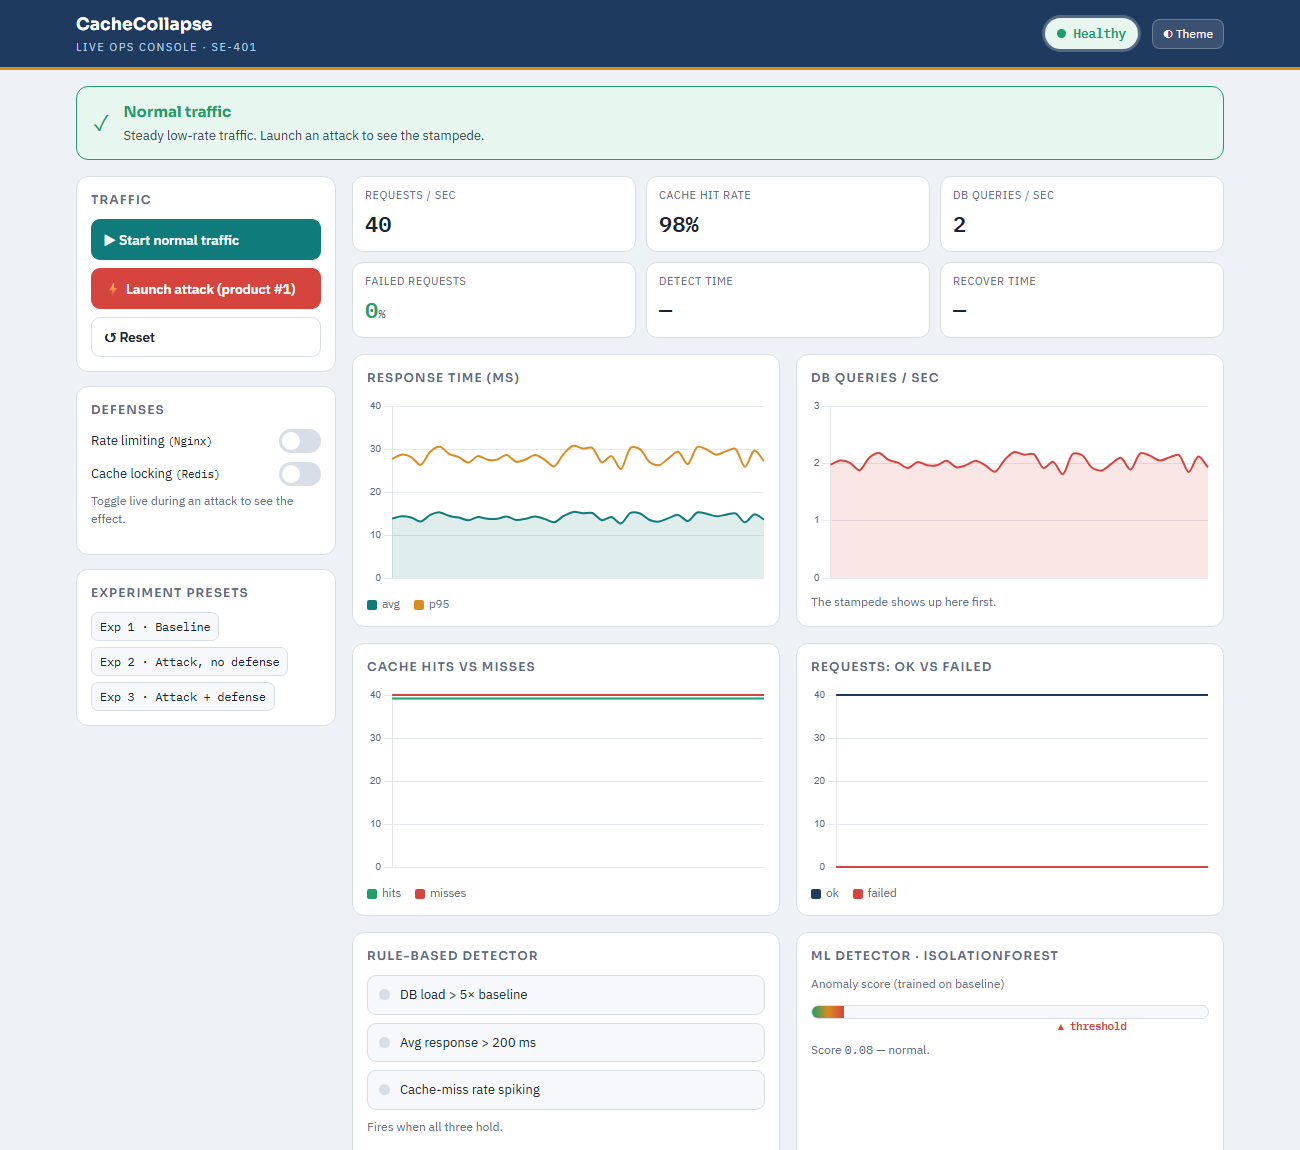
\includegraphics[width=\linewidth]{figures/ui-baseline.png}
\caption{Baseline}
\end{subfigure}\hfill
\begin{subfigure}[t]{0.32\linewidth}\centering
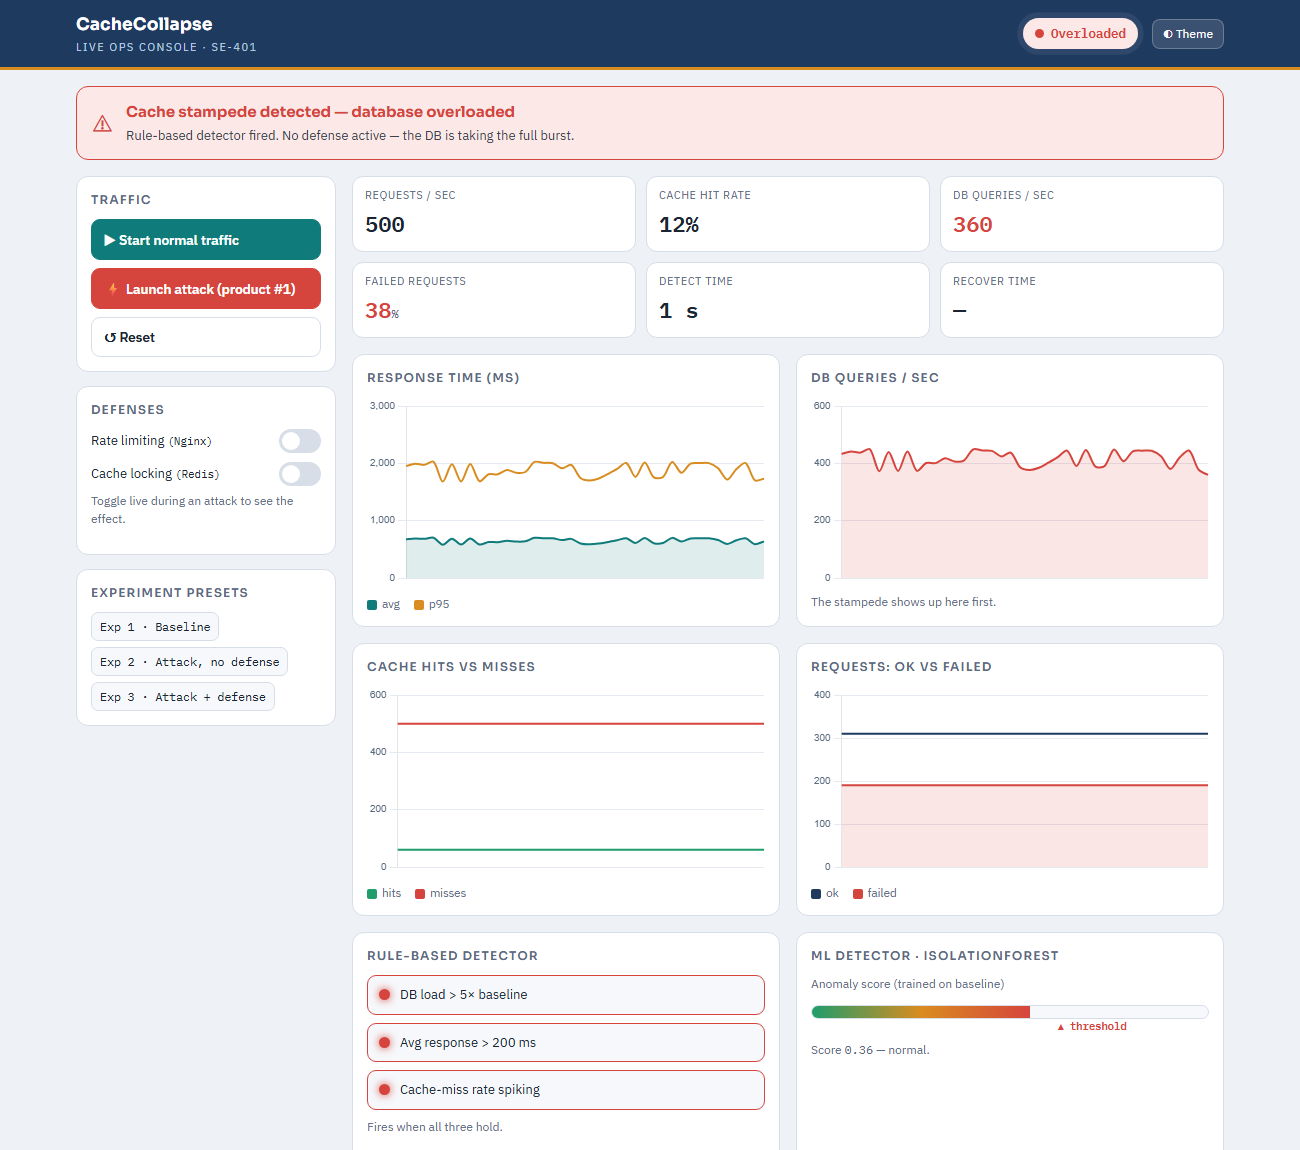
\includegraphics[width=\linewidth]{figures/ui-attack.png}
\caption{Attack, no defense}
\end{subfigure}\hfill
\begin{subfigure}[t]{0.32\linewidth}\centering
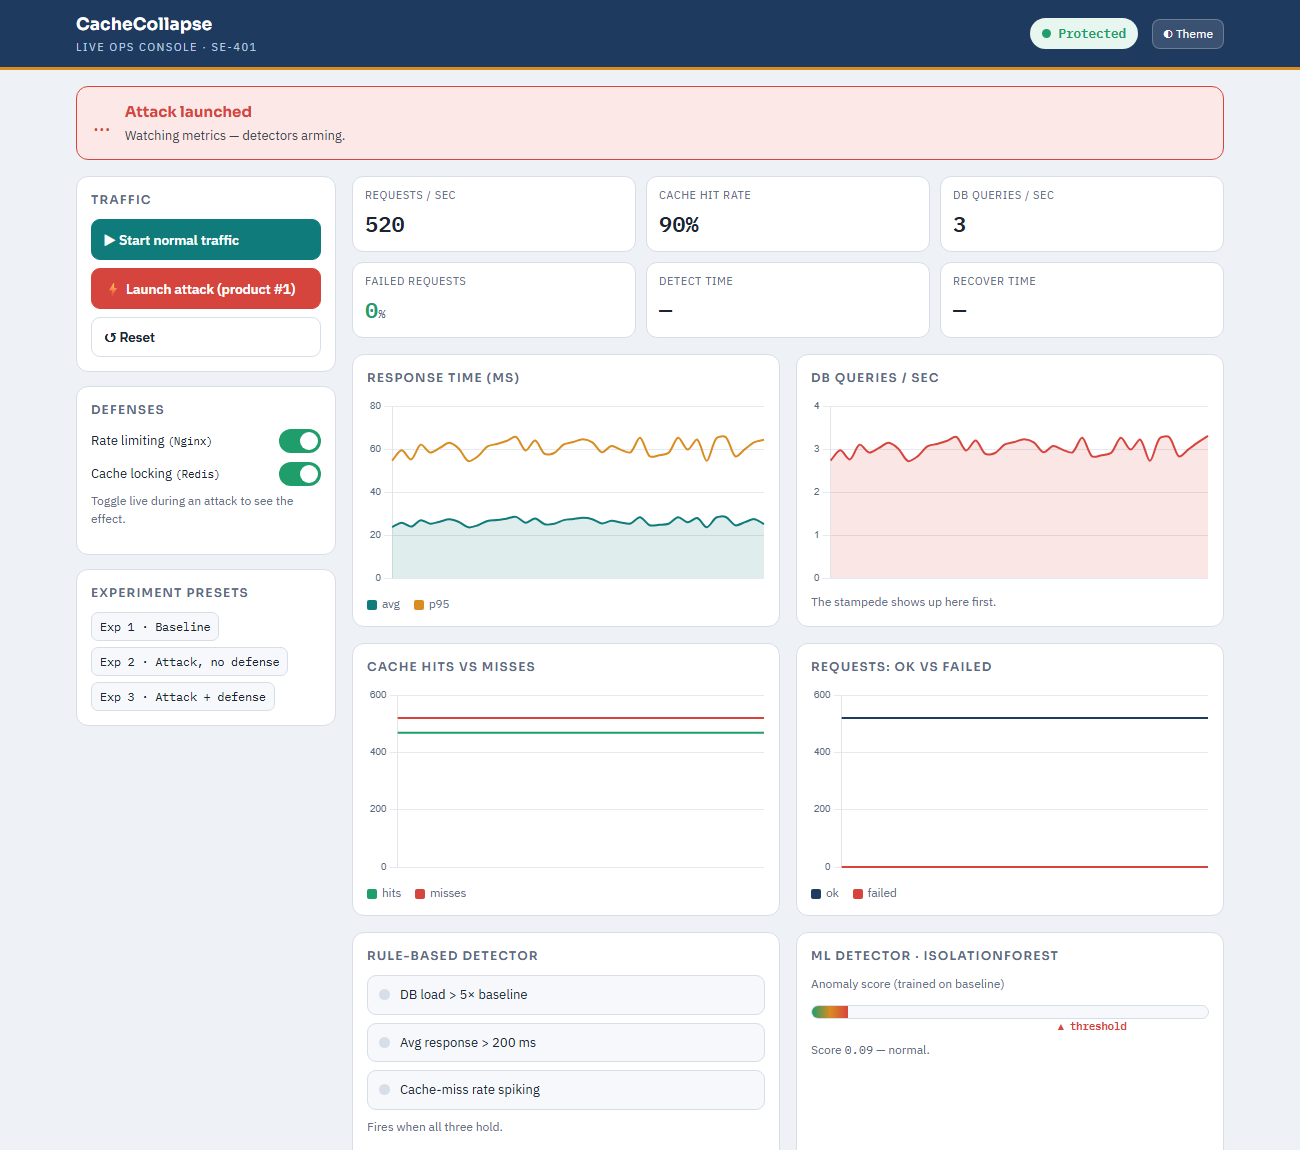
\includegraphics[width=\linewidth]{figures/ui-protected.png}
\caption{Attack with defenses}
\end{subfigure}
\caption{The live operations console in its three demonstration states. These are
\emph{design-phase mockup} screenshots driven by synthetic values to illustrate the
layout; they are not measurements. All quantitative results in this paper come from
the monitor's logs (Section~\ref{sec:results}).}
\label{fig:ui}
\end{figure}

\subsection{Configuration Parameters}
Table~\ref{tab:params} lists every tunable parameter and the value used in the final
configuration. Several values were changed during development (for example the TTL,
which the specification initially set to 10~s); the table reflects the code and
environment used for the results in Section~\ref{sec:results}.

\begin{table}[t]
\centering
\caption{Configuration parameters of the final configuration.}
\label{tab:params}
\small
\begin{tabularx}{\linewidth}{@{}L{4.4cm}L{2.2cm}Y@{}}
\toprule
Parameter & Value & Where / note \\
\midrule
Cache TTL $T$ & 4 s & \texttt{.env} \texttt{CACHE\_TTL}; short so stampedes recur \\
Stale TTL & $15T=60$ s (3{,}600 s pre-warm) & \texttt{app.py} \\
Simulated query time $d_0$ & 110 ms & \texttt{.env} \texttt{DB\_QUERY\_DELAY\_MS} \\
DB pool size $c$ (min) & 12 (2) & \texttt{db.py}; fail-fast \\
Lock expiry / loser poll / max wait & 3{,}000 / 50 / 1{,}500 ms & \texttt{app.py} \\
App rate limit $R$ & 50 req/s per client, 1 s window & \texttt{.env} \texttt{RATE\_LIMIT\_RPS} \\
Edge rate limit & 50 r/s, burst 20, \texttt{nodelay} & \texttt{nginx.conf} + dynamic include \\
Gunicorn (app) & 1 worker $\times$ 200 threads & \texttt{backend/Dockerfile} \\
Products $K$ & 100 & \texttt{seed.sql} \\
Normal traffic & 4 req/batch, 100 ms sleep ($\approx$18 req/s) & \texttt{loadgen.py} \\
Attack burst $B$ / hot pool $H$ / pause & 250 / 20 / 50 ms & \texttt{loadgen.py} \\
Monitor interval $\Delta$ & 0.5 s & \texttt{monitor/app.py} \\
Warm-up suppression $W$ & 6 intervals (3 s) & \texttt{monitor/app.py} \\
Rule: $K$, $\tau_L$, $\tau_m$, floor & 5, 200 ms, 0.5, 5 q/s & \texttt{detect\_rules.py} \\
Baseline EWMA weight & 0.2 & \texttt{monitor/app.py} \\
iForest: min train / window / contamination & 10 / 300 / 0.01 & \texttt{detect\_ml.py} \\
ML debounce & 2 consecutive intervals & \texttt{monitor/app.py} \\
Prometheus scrape interval & 2 s & \texttt{prometheus.yml} \\
\bottomrule
\end{tabularx}
\end{table}

\subsection{Reproducibility and Safe Operation}
The entire system starts with \texttt{docker compose up --build}; the database waits
for a \texttt{pg\_isready} health check before the application starts; and all
configuration is in version-controlled files plus a local \texttt{.env} that is
excluded from version control. The load generator targets only the stack's own proxy
on the private network, so attack traffic never leaves the host. The control endpoints
are deliberately unauthenticated for classroom demonstration; any deployment reachable
by others must restrict access, as discussed in Section~\ref{sec:ethics}. Appendix~A
gives a step-by-step reproduction guide.

%% =====================================================================
\section{Experimental Methodology}
\label{sec:method}
%% =====================================================================

\subsection{Environment}
All experiments ran on a single Windows~11 Pro workstation under Docker Desktop
(Docker Engine 29.8.2), with the nine containers of Table~\ref{tab:services} on one
Compose bridge network. Container resource limits were left at Docker Desktop defaults.
Running every component on one host removes network variability between tiers and
makes runs comparable, at the cost of shared CPU contention between the attacker,
the victim, and the instrumentation (Section~\ref{sec:validity}).

\subsection{Experimental Conditions and Protocol}
Experiments follow a three-condition protocol, executed from the dashboard presets:
\begin{description}[leftmargin=1.2em,style=nextline]
\item[E1 -- Baseline.] Normal traffic only, defenses off.
\item[E2 -- Attack, undefended.] Normal traffic plus the rotating burst attack, both
defenses off.
\item[E3 -- Attack, defended.] Normal traffic plus the attack, with cache locking,
application rate limiting, and edge rate limiting enabled.
\end{description}
A typical session cycles E1~$\rightarrow$~E2~$\rightarrow$~E1~$\rightarrow$~E3 with
roughly 5--20~s per condition, so that each undefended and each defended attack is
preceded by a fresh normal period from which the detectors can (re)learn the
baseline. In addition, the final session contains one long defended run spanning
${\approx}8.1$~h of wall-clock time, used as a soak test of the defense; it contains
4.5~h of valid samples, the remainder being 15 gaps during which the host was asleep.
Two further procedures were used:
\begin{itemize}[leftmargin=*]
\item \textbf{Ablation.} Starting from E2, defenses were enabled one at a time (cache
locking only; plus stale-while-revalidate; plus edge rate limiting) while observing the
dashboard and the CacheShop storefront (Section~\ref{sec:ablation}). Because the
defense implementation evolved during the project, the 14 sessions that include
defended traffic also form a natural longitudinal ablation, analyzed in
Section~\ref{sec:longitudinal}.
\item \textbf{Automated validation.} A 16-case end-to-end test suite drives the system
through the same control API and checks functional and quantitative success criteria
(Section~\ref{sec:validation}).
\end{itemize}

\subsection{Dataset}
The monitor writes one CSV row per sampling interval (Table~\ref{tab:csv}). A new file
is started each time the monitor container boots. The study uses all 18 files produced
on 22~October~2026, totalling 92{,}531 rows and ${\approx}28$~h of wall-clock logging,
much of it idle (Table~\ref{tab:dataset}). The sampling interval was 1~s in the first
eight sessions and 0.5~s thereafter.

\begin{table}[t]
\centering
\caption{Columns of the monitor's CSV log (one row per sampling interval).}
\label{tab:csv}
\small
\begin{tabularx}{\linewidth}{@{}L{2.6cm}Y@{}}
\toprule
Column & Definition \\
\midrule
\texttt{ts} & Unix timestamp of the sample \\
\texttt{mode} & idle / normal / attack / protected (attack with $\ge$1 defense on) \\
\texttt{rps} & Application requests per second (all outcomes, incl.\ 429 and 503) \\
\texttt{db\_qps} & Database query \emph{attempts} per second \\
\texttt{cache\_hits}, \texttt{cache\_misses} & Counts in the interval \\
\texttt{hit\_rate} & hits / (hits + misses) in the interval \\
\texttt{resp\_avg\_ms} & Mean in-application latency of requests completed in the interval \\
\texttt{resp\_p95\_ms} & Histogram-bucket approximation of p95 latency \\
\texttt{failed} & \emph{Count} of HTTP~503 responses in the interval (not a rate) \\
\texttt{rule\_alert}, \texttt{ml\_alert} & Detector outputs (0/1) \\
\texttt{ml\_score} & Normalized anomaly score for display (0.08 = model not yet trained) \\
\bottomrule
\end{tabularx}
\end{table}

\begin{table}[t]
\centering
\caption{Dataset summary. ``Final'' is the session with the complete defense
(edge rate limiting active), on which the main results are computed.}
\label{tab:dataset}
\small
\begin{tabular}{@{}lrrrrr@{}}
\toprule
Subset & Rows & Idle & Normal & Attack & Defended \\
\midrule
All 18 sessions & 92{,}531 & 50{,}732 & 1{,}477 & 1{,}648 & 38{,}674 \\
Final session (16:58), valid rows & 61{,}923 & 25{,}586 & 332 & 733 & 35{,}272 \\
\bottomrule
\end{tabular}
\end{table}

\paragraph{Choice of the primary dataset.} The defense evolved during the day
(Section~\ref{sec:lessons}). Only in the last session is the edge rate limiter
demonstrably active: the application's request rate in defended mode is pinned at the
configured 50~req/s (median 50, IQR 47--53), whereas in every earlier session it is
170--350~req/s. We therefore report the main results on the final session (12
undefended attack episodes totalling 13~min of valid samples, 10 defended episodes
totalling 5.6~h of which 4.5~h are the soak run, and 12 normal episodes) and use the earlier sessions for the longitudinal
analysis and for robustness checks.

\subsection{Pre-processing}
\begin{enumerate}[leftmargin=*]
\item \textbf{Interval length.} For each row, $\Delta t$ is the difference between
consecutive timestamps. Rows with $\Delta t\notin(0.25, 2.0)$~s are excluded (245 of
92{,}531 rows, 0.26\%). These arise when the host sleeps or the monitor stalls and produce
meaningless rates; for example one such row in the soak run reports a mean latency of
over 1{,}000~s.
\item \textbf{Failure rate.} Because \texttt{failed} is a per-interval count, the
failure rate is computed as $\texttt{failed}/\Delta t$.
\item \textbf{Miss ratio.} Computed as misses/(hits+misses) per interval, 0 when both
are zero.
\item \textbf{Episodes.} Each maximal run of consecutive rows with the same mode is an
\emph{episode}. Episodes shorter than 8 rows are excluded from per-episode analyses
(they are transitions caused by rapid button presses).
\item \textbf{ML readiness.} Rows with \texttt{ml\_score}$=0.08$ and no ML alert are
those in which the forest had not yet been trained; per-episode ML results report
whether the model was ready.
\end{enumerate}

\subsection{Ground Truth and Evaluation Metrics}
The mode recorded in each row provides ground truth: intervals in \emph{attack} mode
are positives (the attack is running and undefended) and intervals in \emph{normal}
mode are negatives. Defended and idle intervals are reported separately, because the
correct answer there is a matter of definition: during a defended attack the attack
\emph{is} present but causes no harm, and during idle periods there is no traffic at
all. Table~\ref{tab:metric-defs} defines the evaluation metrics.

\begin{table}[t]
\centering
\caption{Evaluation metrics.}
\label{tab:metric-defs}
\small
\begin{tabularx}{\linewidth}{@{}L{3.6cm}Y@{}}
\toprule
Metric & Definition \\
\midrule
DB load & Median (IQR, p95, max) of \texttt{db\_qps} over intervals in a condition \\
Latency & Median (IQR, p95, max) of per-interval mean latency \\
Failure rate & HTTP 503 per second; fraction of intervals with any 503 \\
Reduction factor & Ratio of medians (undefended / defended), 95\% bootstrap CI \cite{efron1994} \\
Coalescing ratio $\rho$ & Total cache misses / total DB attempts in a condition \\
Completed DB queries & $\max(0, q_{db}\Delta t - n_{503})/\Delta t$ per interval \\
Detection latency & Time from first interval of an attack episode to first alert \\
Episode recall & Fraction of attack episodes with at least one alert \\
Interval precision / recall / F1 & Over attack (positive) and normal (negative) intervals \\
False-positive rate & Alerts in normal intervals / normal intervals \\
ROC AUC & Area under the ROC curve of a continuous score \cite{fawcett2006} \\
Recovery time & First interval of a new condition to the first of two consecutive healthy intervals (Eq.~\ref{eq:healthy}) \\
\bottomrule
\end{tabularx}
\end{table}

\subsection{Offline Analyses}
Three analyses go beyond the detectors' live output.
\begin{itemize}[leftmargin=*]
\item \textbf{Threshold sensitivity of the rule.} Equation~\eqref{eq:rule} is
re-evaluated on the logged features over a grid of $K\in\{2,3,5,8,12\}$,
$\tau_L\in\{100,150,200,300\}$~ms and $\tau_m\in\{0.3,0.5,0.7\}$, using the median
normal database rate of the final session (11~q/s) as baseline.
\item \textbf{Single-signal baselines.} Each condition of the rule, a ``failures
present'' detector, and a pure volume threshold (rps$\,>100$) are evaluated alone, both
on the attack/normal intervals and on 2{,}080 \emph{absorbed-burst} intervals: defended
intervals from six earlier sessions in which the full attack volume reached the
application (median 280~req/s) but was served from cache with low database load
(median 2~q/s) and low latency (median 26~ms). These are high-volume, harmless
intervals---a laboratory proxy for a flash crowd that the cache absorbs.
\item \textbf{Offline IsolationForest replay.} The detector pipeline is re-run offline
with the same features, scaler, and hyper-parameters: it is trained on the first half
of the final session's normal intervals (166) and tested on the second half (166) plus
all 733 attack intervals. This permits ROC analysis, a sweep of the
\texttt{contamination} parameter, a sweep of the training-window size, and a
random-seed stability check.
\end{itemize}
All analysis code uses pandas, NumPy, scikit-learn, and Matplotlib, and reads only the
CSV logs.

%% =====================================================================
\section{Results}
\label{sec:results}
%% =====================================================================

Unless stated otherwise, results are computed on the valid intervals of the final
session; ``median (IQR)'' denotes the median and interquartile range over sampling
intervals.

\subsection{Cache Behavior (Sanity Check)}
\label{sec:sanity}
The first request for a product is answered from the database in ${\approx}137$--$180$~ms
across runs, and an immediate repeat is answered from Redis in ${\approx}9$--$12$~ms
(test case~5 measured 137~ms and 9~ms). The roughly fifteen-fold difference between a
hit and a miss confirms that the cache is the component under contention during a
stampede and, as noted in Section~\ref{sec:recon}, that cache state is externally
observable through timing.

\subsection{Baseline Behavior and Validation of the Analytical Model (RQ2)}
\label{sec:baseline}
Under normal traffic the application receives a median of 18~req/s (IQR 16--19),
issues 11~database queries/s (IQR 9--14), and serves requests with a median
per-interval mean latency of 77~ms (IQR 61--94); only 2 HTTP~503 responses occur in
332 normal intervals. Figure~\ref{fig:baseline-model} compares the measured database
rate with the prediction of Eq.~\eqref{eq:baseline}. Across 725 normal intervals from
all sessions sampled at 0.5~s, the median request rate is $\lambda=17$~req/s, for which
the model predicts $q_{\mathrm{base}}=10.1$~q/s and a miss ratio of 0.60; the measured
medians are 11.0~q/s and 0.63. The model therefore predicts baseline database load to
within 9\% using only the catalog size, the TTL, and the request rate, and it explains
a result that surprises many readers: \emph{under a short TTL and a uniform catalog,
the normal miss ratio is already above one half}. This fact shapes the detection
results in Section~\ref{sec:det-results}.

\begin{figure}[t]
\centering
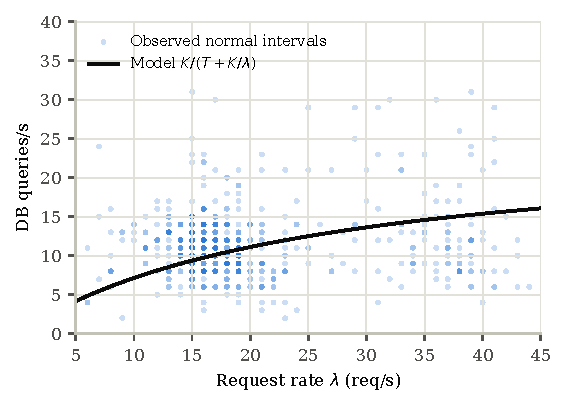
\includegraphics[width=0.62\linewidth]{figures/fig_baseline_model.pdf}
\caption{Baseline database load versus request rate. Points are normal-traffic
intervals from all sessions; the line is the analytical prediction
$q_{\mathrm{base}}=K/(T+K/\lambda)$ with $K=100$ and $T=4$~s
(Eq.~\ref{eq:baseline}).}
\label{fig:baseline-model}
\end{figure}

\subsection{Three-Condition Comparison (RQ1, RQ4)}
\label{sec:three}
Table~\ref{tab:three} reports the distribution of each metric under the three
conditions, and Figure~\ref{fig:timeline} shows one representative cycle of
normal~$\rightarrow$~undefended attack~$\rightarrow$~normal~$\rightarrow$~defended
attack.

\begin{table}[t]
\centering
\caption{Three-condition comparison on the final session. Values are median (IQR) over
sampling intervals, with p95 and maximum where informative. Failures are HTTP~503 per
second. $n$ is the number of intervals.}
\label{tab:three}
\small
\begin{tabularx}{\linewidth}{@{}L{3.3cm}YYY@{}}
\toprule
Metric & E1 Baseline & E2 Attack, undefended & E3 Attack, defended \\
& ($n=332$) & ($n=733$) & ($n=35{,}272$) \\
\midrule
Requests/s at app & 18 (16--19) & 250 (206--298) & 50 (47--53) \\
DB attempts/s & 11 (9--14) & 108 (51--150) & 6 (4--8) \\
\quad p95 / max & 17 / 34 & 205 / 317 & 12 / 174 \\
Mean latency (ms) & 77 (61--94) & 174 (101--256) & 27 (20--37) \\
\quad p95 / max & 122 / 199 & 450 / 1{,}159 & 84 / -- \\
503 failures/s & 0 (0--0) & 84 (35--124) & 0 (0--0) \\
\quad p95 / max & 0 / 3.9 & 173 / 274 & 0 / 154 \\
Intervals with any 503 & 0.3\% & 79.7\% & $<$0.01\% \\
Cache-miss ratio & 0.62 (0.50--0.75) & 0.51 (0.31--0.59) & 0.42 (0.32--0.50) \\
Coalescing ratio $\rho$ & 1.00 & 1.00 & 4.70 \\
Completed DB queries/s & 11 & 23 & 6 \\
Status & Healthy & Overloaded & Protected \\
\bottomrule
\end{tabularx}
\end{table}

\begin{figure}[t]
\centering
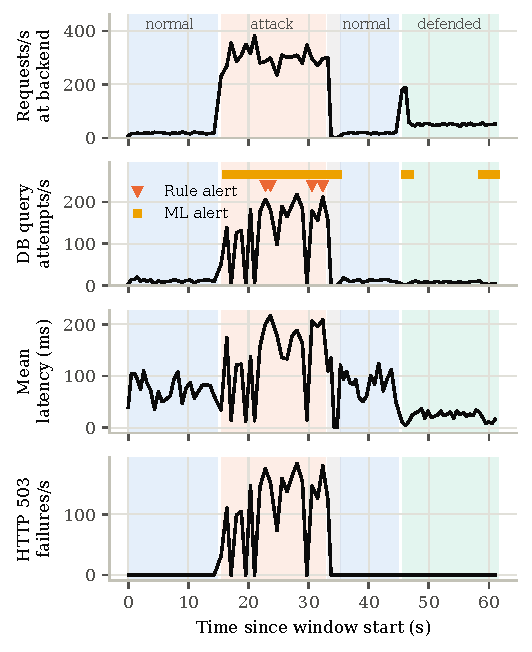
\includegraphics[width=0.92\linewidth]{figures/fig_timeline.pdf}
\caption{A representative 60~s window from the final session. Shading marks the mode
(blue: normal; orange: undefended attack; green: attack with all defenses; grey: brief
idle). Triangles and squares above the second panel mark intervals in which the rule
and the IsolationForest raised alerts.}
\label{fig:timeline}
\end{figure}

\paragraph{Undefended attack (E2).} The attack raised the application's request rate
from 18 to a median of 250~req/s and the rate of database query attempts from 11 to a
median of 108/s (9.8$\times$ the baseline median), with a peak of 317/s (28.8$\times$).
Median latency more than doubled to 174~ms, with a p95 of 450~ms and a maximum of
1.16~s, and 79.7\% of intervals contained HTTP~503 failures, at a median of 84
failures/s and up to 274/s. Of 77{,}408 database attempts, 61{,}336 (79\%) were
rejected because the pool was exhausted. This is a clear denial of service produced
entirely by well-formed requests for existing products.

\paragraph{Defended attack (E3).} With all defenses enabled, the same attack left the
database at a median of 6~q/s (IQR 4--8, p95 12)---\emph{below} the normal baseline of
11~q/s, because the edge limiter also throttles the normal traffic from the shared
load-generator address (Section~\ref{sec:validity}). The application's request rate
was pinned at the edge limiter's 50~req/s, median latency fell to 27~ms (p95 84~ms),
and failures were effectively eliminated: 419 HTTP~503 responses in 35{,}272 intervals,
concentrated in a handful of intervals at mode transitions. The defended database load
of 6~q/s is in line with the analytical bound of Eq.~\eqref{eq:defended}
($H/T=5$~q/s for the hot keys plus a small residue of normal misses).

\paragraph{Effect sizes.} The ratio of median database load, undefended to defended,
is 18.0$\times$ (95\% bootstrap CI 16.8--19.2$\times$); the ratio of means is
16.0$\times$. The ratio of median latency is 6.4$\times$ (CI 6.1--6.8$\times$).
Comparing a \emph{peak} undefended value with a \emph{typical} defended value would
give much larger factors (e.g.\ $317/6\approx53\times$); we report ratios of medians
because they are robust to the bursty, heavy-tailed behavior of the attack and are
therefore the more conservative and defensible statistic.

\paragraph{Distributions.} Figure~\ref{fig:boxplots} shows the full distributions and
Figure~\ref{fig:cdf} the latency CDFs. The defended latency distribution lies almost
entirely to the left of the baseline distribution (their interquartile ranges, 20--37~ms
and 61--94~ms, do not overlap): with stale-while-revalidate, most requests are
served from Redis in a few milliseconds, whereas in the baseline many requests are
genuine misses costing ${\geq}110$~ms. Defended service is thus not merely ``restored''
but \emph{faster than normal}, at the price of serving data up to one stale TTL old.

\begin{figure}[t]
\centering
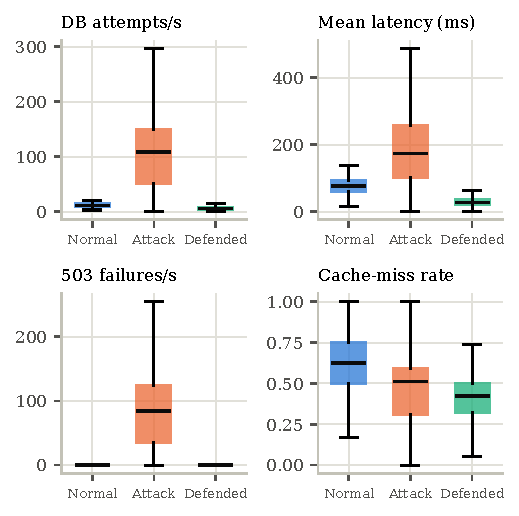
\includegraphics[width=\linewidth]{figures/fig_boxplots.pdf}
\caption{Per-interval distributions under the three conditions (final session; boxes
show IQR, whiskers 1.5$\times$IQR, outliers omitted).}
\label{fig:boxplots}
\end{figure}

\begin{figure}[t]
\centering
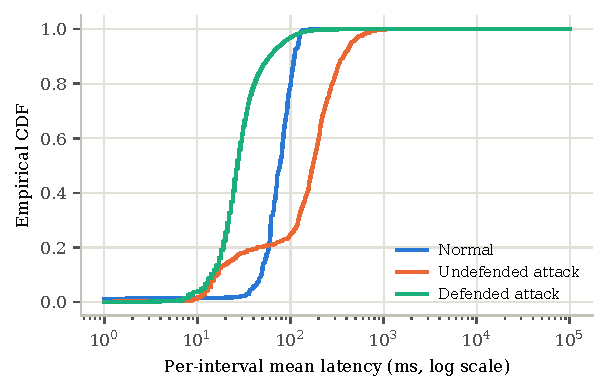
\includegraphics[width=0.66\linewidth]{figures/fig_latency_cdf.pdf}
\caption{Empirical CDF of per-interval mean latency (log scale).}
\label{fig:cdf}
\end{figure}

\paragraph{Soak test.} During the 4.5~h of valid samples in the long defended run, the
median database load was 6~q/s (p99 15), median latency 27~ms (p99 140~ms), and only a
single interval contained failures. The defense is therefore stable over hours, not
just over a demonstration-length run.

\subsection{Overload Mechanics: Why the Stampede Becomes a Denial of Service (RQ2)}
\label{sec:mechanics}
Figure~\ref{fig:saturation} plots, for every interval, the HTTP~503 rate against the
rate of database attempts. Undefended intervals lie on a line of slope close to one,
offset by roughly 20--25 attempts per second: beyond a small number of attempts per
second, \emph{every additional attempt fails}. Equivalently, the rate of
\emph{completed} database queries during the attack has a median of only 23/s---barely
twice the baseline and about one fifth of the nominal pool capacity
$\mu_{\max}=c/d_0\approx109$~q/s of Eq.~\eqref{eq:mu}.

\begin{figure}[t]
\centering
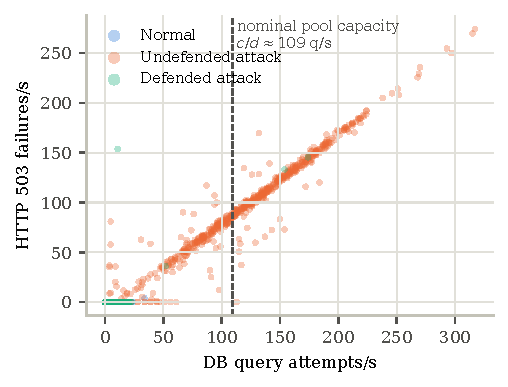
\includegraphics[width=0.66\linewidth]{figures/fig_db_saturation.pdf}
\caption{HTTP 503 failures/s versus database query attempts/s per interval. Under the
undefended attack, failures grow one-for-one with attempts once a small completed
throughput is reached, far to the left of the nominal pool capacity (dashed line).}
\label{fig:saturation}
\end{figure}

Three mechanisms, each visible in the design, explain this goodput collapse
\cite{jacobson1988,mogul1997}. First, the pool is \emph{fail-fast}
(Section~\ref{sec:bg-queueing}), so a burst of $B=250$ simultaneous misses can obtain at
most 12 connections and the rest fail at once rather than queueing. Second, failed
regenerations do not populate the cache, so a request arriving 10~ms later misses again
and makes another doomed attempt; the burst keeps re-stampeding the same key until one
query completes. Third, all 200 application threads share one Python interpreter, so
the bookkeeping of hundreds of concurrent failing requests competes for CPU with the
few that hold connections, lengthening the effective connection-holding time beyond
$d_0$. The analytical model's capacity bound is therefore optimistic by a factor of
roughly four, and the practical lesson is that \emph{the database is overwhelmed long
before its nominal capacity is reached}, because the stampede wastes the very
resource it contends for.

\subsection{Mitigation Effectiveness and Coalescing (RQ4)}
\label{sec:mitigation-results}
The coalescing ratio $\rho$ (misses per database attempt) makes the effect of locking
directly visible. Without locking, $\rho=1.00$ in both normal and attack conditions:
every miss becomes a database attempt. With locking, $\rho=4.70$ over 592{,}029 misses
and 125{,}957 database attempts: on average almost five concurrent misses were served
by one regeneration. Because losers are served the stale copy, the misses also do not
wait; the median defended latency of 27~ms is close to pure cache-hit time plus
proxy overhead. The edge limiter's effect is equally visible: the median application
request rate under attack falls from 250~req/s to exactly the configured 50~req/s.

\subsection{Mitigation Ablation}
\label{sec:ablation}
Table~\ref{tab:ablation} summarizes the ablation performed by enabling defenses one at a
time during an attack and observing the dashboard and the CacheShop storefront, and
links each step to the corresponding measured evidence.

\begin{table}[t]
\centering
\caption{Mitigation ablation (customer-visible behavior under attack). Storefront
latencies are per-item load times observed on CacheShop; DB load from the logs.}
\label{tab:ablation}
\small
\begin{tabularx}{\linewidth}{@{}L{3.4cm}L{2.5cm}L{3.1cm}L{1.8cm}Y@{}}
\toprule
Configuration & DB load & Storefront & Availability & Evidence \\
\midrule
No defense & Overloaded (median 108 attempts/s) & Fails or 300--500~ms & Denied & Table~\ref{tab:three} \\
Cache lock only (losers wait) & Protected (1--4 q/s) & Slow; up to ${\approx}2.5$~s queuing & Degraded & Bug 4, sessions 11:05--12:57 \\
+ Stale-while-revalidate & Protected & 80--140~ms, still variable & Degraded (proxy congested) & Bug 4 fix; sessions from 13:34 \\
+ Edge rate limiting & Protected (6 q/s) & 20--140~ms & Preserved & Bug 6 fix; final session \\
\bottomrule
\end{tabularx}
\end{table}

The central finding is that \emph{database protection and request-path protection are
distinct problems requiring distinct controls}. Cache locking alone protects the
database---query load drops to single digits because $N$ misses are coalesced to
one---but does not by itself keep users fast. In the first implementation losers
waited for the winner, and protected-mode latency reached ${\approx}2.5$~s;
stale-while-revalidate removed that queue. Even then, the attacker's full volume still
reached the proxy and the application: with only application-layer controls, every
attack request still consumed a proxy connection and an application thread, and the
storefront stayed slow and variable even though the database was healthy. Only edge
rate limiting, which rejects the flood at the proxy before it consumes upstream
resources, made storefront latency consistently low.

\subsection{Longitudinal Analysis of the Defense}
\label{sec:longitudinal}
Because the defense was improved during the day, the 14 sessions containing defended
traffic form a natural experiment (Figure~\ref{fig:dev}). In the first three sessions
(11:05--11:16) the median defended latency was 105--107~ms; in the next four
(11:20--12:57) 65--91~ms; from 13:34 onwards, once the stale-while-revalidate path
and real client-address forwarding were in place, it fell to 26--32~ms (42--49~ms in
two sessions that contained only defended traffic), a three- to four-fold improvement
that is stable across sessions. The lower panel shows the second
step: until the final session the application still received 170--350~req/s under a
defended attack, i.e.\ the full attack volume passed the proxy; in the final session,
with edge limiting active, it is pinned at 50~req/s. Meanwhile, undefended attacks
remained severe in every session (median latency 96--351~ms), confirming that the
improvement is due to the defense and not to a weaker attack. The first defended run
(11:05) is the only one with a substantial failure rate (146/s on average); the later
runs, and the decision recorded in the development log to count HTTP~429
(intentional shedding) separately from HTTP~503 (overload), indicate that this was an
artefact of an early version rather than a property of the defense.

\begin{figure}[t]
\centering
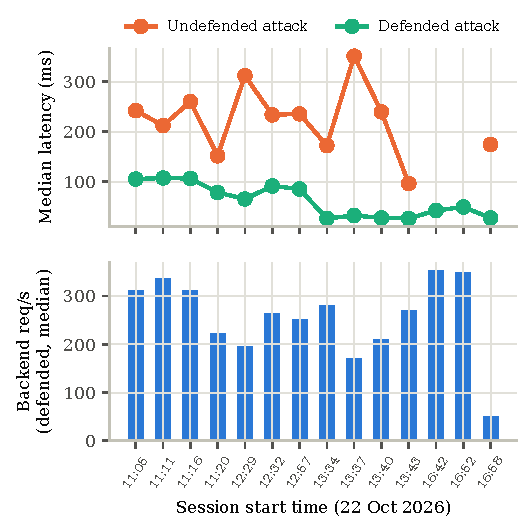
\includegraphics[width=0.92\linewidth]{figures/fig_dev_evolution.pdf}
\caption{Longitudinal view of 14 sessions. Top: median per-interval latency under
undefended and defended attack. Bottom: median request rate reaching the application
during defended attack; only in the final session does the edge limiter cap it at
50~req/s. The 16:42 and 16:52 sessions contained no undefended attack.}
\label{fig:dev}
\end{figure}

\subsection{Recovery (RQ4)}
\label{sec:recovery}
Recovery time is measured from the first interval of the new condition until the first
of two consecutive healthy intervals (Eq.~\ref{eq:healthy}). Across all sessions,
when defenses were enabled during an ongoing attack (7 transitions), the system became
healthy after a median of 1.35~s (maximum 2.77~s); in the final session the three such
transitions took 0.75, 1.35, and 1.50~s. When the attack was stopped (31 transitions),
26 recovered within the following episode, after a median of 1.08~s (maximum 2.51~s);
the remainder were followed by episodes too short to observe two healthy intervals.
Recovery is fast because cache locking immediately collapses redundant queries and the
pre-warmed stale cache serves losers without waiting, while the edge limiter's
configuration change takes effect within the watcher's one-second polling period. The
end-to-end test suite independently measured recovery after an attack stops at
${\approx}2$~s.

\subsection{Detection: Rule-Based versus IsolationForest (RQ3)}
\label{sec:det-results}

\paragraph{Per-episode detection.} Table~\ref{tab:episodes} lists the 12 undefended
attack episodes of the final session and Figure~\ref{fig:detlat} summarizes detection
latency. The rule detected 11 of 12 episodes with a median latency of 3.2~s (IQR
2.4--5.6~s, maximum 18.1~s). The IsolationForest detected 10 of 12 with a median
latency of 0.85~s (IQR 0--1.0~s, maximum 1.3~s). One ML miss occurred in the very first
attack of the session, before any normal traffic had been seen and therefore before
the model existed; the other occurred immediately after the model had been trained
for the first time on a short baseline. The two detectors' misses do not overlap, so
their union detected \emph{all 12 episodes}, with a median latency of 0.95~s.
Detection latencies of 0.0~s mean the alert was already raised in the first interval
labelled ``attack'', because traffic changes slightly before the monitor reads the new
mode flag.

\begin{table}[t]
\centering
\caption{Per-episode detection on the 12 undefended attack episodes of the final
session. $t$ = time from onset to first alert; cov.\ = fraction of the episode's
intervals with an alert; --- = not detected.}
\label{tab:episodes}
\small
\begin{tabular}{@{}rrrrrrrrr@{}}
\toprule
\# & Intervals & Duration (s) & DB med. & Latency med. & \multicolumn{2}{c}{Rule} & \multicolumn{2}{c}{IsolationForest} \\
\cmidrule(lr){6-7}\cmidrule(lr){8-9}
 & & & (q/s) & (ms) & $t$ (s) & cov. & $t$ (s) & cov. \\
\midrule
1 & 20 & 15.8 & 141 & 111 & 2.5 & 0.20 & ---$^\dagger$ & 0.00 \\
2 & 21 & 17.1 & 172 & 159 & 2.8 & 0.19 & --- & 0.00 \\
3 & 13 & 8.9 & 175 & 83 & --- & 0.00 & 0.0 & 0.31 \\
4 & 17 & 16.0 & 152 & 204 & 3.2 & 0.41 & 0.9 & 0.94 \\
5 & 21 & 16.9 & 165 & 158 & 7.4 & 0.19 & 1.0 & 0.95 \\
6 & 12 & 8.7 & 180 & 141 & 2.3 & 0.08 & 0.0 & 1.00 \\
7 & 22 & 17.5 & 188 & 142 & 1.0 & 0.09 & 1.0 & 0.95 \\
8 & 14 & 9.8 & 175 & 119 & 3.7 & 0.07 & 0.0 & 1.00 \\
9 & 65 & 53.2 & 58 & 37 & 18.1 & 0.08 & 0.8 & 0.95 \\
10 & 30 & 25.7 & 129 & 112 & 2.3 & 0.17 & 1.3 & 0.97 \\
11 & 474 & 562.1 & 100 & 209 & 3.2 & 0.35 & 0.0 & 1.00 \\
12 & 31 & 33.8 & 92 & 126 & 9.5 & 0.23 & 1.1 & 0.87 \\
\midrule
\multicolumn{5}{@{}l}{Detected / median $t$} & 11/12 & 3.2 s & 10/12 & 0.85 s \\
\bottomrule
\multicolumn{9}{@{}l}{\footnotesize $^\dagger$Model not yet trained (no normal traffic had been observed).}
\end{tabular}
\end{table}

\begin{figure}[t]
\centering
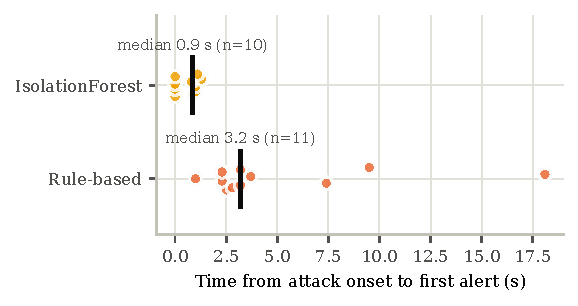
\includegraphics[width=0.66\linewidth]{figures/fig_detect_latency.pdf}
\caption{Detection latency per attack episode (final session). Vertical bars mark
medians.}
\label{fig:detlat}
\end{figure}

\paragraph{Interval-level accuracy.} Table~\ref{tab:tick} reports interval-level
metrics over 733 attack and 332 normal intervals. The rule is perfectly precise (no
false positives) but fires on only 27\% of attack intervals, because the stampede is
bursty and its three conditions coincide only intermittently. The IsolationForest
fires on 91\% of attack intervals (94\% once trained) with a single false positive in
332 normal intervals (FPR 0.3\%), giving an F1 of 0.95. Combining them with a logical
OR yields recall 0.93 and F1 0.96 at the same false-positive rate.

\begin{table}[t]
\centering
\caption{Interval-level detection performance, final session (positives: 733 attack
intervals; negatives: 332 normal intervals).}
\label{tab:tick}
\small
\begin{tabular}{@{}lrrrrrrr@{}}
\toprule
Detector & TP & FP & FN & Precision & Recall & F1 & FPR \\
\midrule
Rule (Eq.~\ref{eq:rule}) & 201 & 0 & 532 & 1.000 & 0.274 & 0.430 & 0.000 \\
IsolationForest & 670 & 1 & 63 & 0.999 & 0.914 & 0.954 & 0.003 \\
IsolationForest (model ready) & 670 & 1 & 43 & 0.999 & 0.940 & 0.968 & 0.003 \\
Rule OR IsolationForest & 678 & 1 & 55 & 0.999 & 0.925 & 0.960 & 0.003 \\
\bottomrule
\end{tabular}
\end{table}

\paragraph{Beyond attack and normal: idle and defended traffic.} Table~\ref{tab:alertrates}
shows how often each detector fires in all four modes. The rule fired in 0.01\% of
idle intervals and never in defended intervals. The IsolationForest fired in 99.3\% of
idle intervals and 12.8\% of defended intervals. The idle result is the closed-world
problem of Sommer and Paxson \cite{sommer2010} in miniature: a model that has seen only
``normal traffic'' regards \emph{no traffic} as maximally abnormal. On the dashboard
this appears as a persistent ML alert whenever traffic is stopped. The defended result
is more nuanced: during a defended attack the attack \emph{is} present, so an alert is
arguably correct as a statement about traffic, but no damage is occurring. The two
detectors are therefore answering different questions---the rule asks ``is the
database being harmed?'', the forest asks ``does traffic look unlike what I learned?''.
We return to this distinction in Section~\ref{sec:discussion}.

\begin{table}[t]
\centering
\caption{Fraction of intervals with an alert, by mode (final session).}
\label{tab:alertrates}
\small
\begin{tabular}{@{}lrrrr@{}}
\toprule
Detector & Idle ($n=25{,}586$) & Normal ($n=332$) & Attack ($n=733$) & Defended ($n=35{,}272$) \\
\midrule
Rule & 0.0001 & 0.000 & 0.274 & 0.000 \\
IsolationForest & 0.993 & 0.003 & 0.914 & 0.128 \\
\bottomrule
\end{tabular}
\end{table}

\paragraph{Why the rule is conservative: threshold sensitivity.} Figure~\ref{fig:rulegrid}
re-evaluates the rule over a grid of thresholds (with $\tau_m=0.5$). Recall is governed
almost entirely by the latency threshold $\tau_L$: at the deployed $\tau_L=200$~ms only
27\% of attack intervals qualify, while at $\tau_L=100$~ms 51\% do, and the
false-positive rate stays at or below 0.9\% everywhere on the grid. Across the full
grid (including $\tau_m$), the best F1 of 0.82 (precision 0.99, recall 0.70, FPR 0.9\%)
is obtained with $K=2$, $\tau_L=100$~ms, $\tau_m=0.3$. The deployed thresholds were
chosen during development to give zero false alarms on calm traffic and are
conservative; Figure~\ref{fig:rulegrid} shows there is room to roughly double recall at
a cost of a few false alarms per thousand intervals.

\begin{figure}[t]
\centering
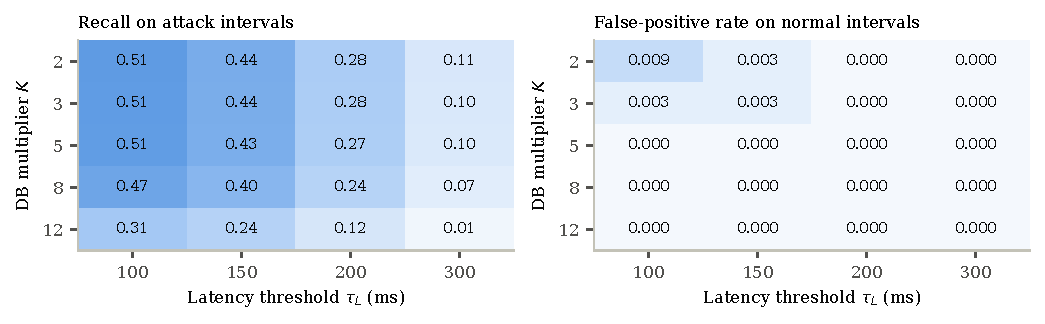
\includegraphics[width=\linewidth]{figures/fig_rule_grid.pdf}
\caption{Threshold sensitivity of the rule (final session, $\tau_m=0.5$). Left: recall
on attack intervals. Right: false-positive rate on normal intervals.}
\label{fig:rulegrid}
\end{figure}

\paragraph{Single-signal baselines and the flash-crowd proxy.} Table~\ref{tab:single}
evaluates each signal alone. On the attack/normal intervals, a pure volume threshold
(rps$\,>100$) looks excellent (recall 0.97, no false positives), because in this
testbed attack traffic is an order of magnitude larger than normal traffic. Its
weakness appears on the 2{,}080 absorbed-burst intervals, in which the full attack
volume reached the application but was served from cache: the volume detector fired on
97.1\% of them, whereas the database-load condition, the failure condition, and the
full rule fired on none. This is the quantitative justification for the multi-signal
design: \emph{volume detects traffic; the rule detects harm}. The table also exposes a
weakness in the rule's third condition. Because the normal miss ratio is already high
(Section~\ref{sec:baseline}), ``miss ratio $>0.5$'' fires on 67\% of normal intervals
and, on its own, is worse than useless; within the conjunction it only removes true
positives. The database-load condition alone (F1 0.85) and the presence of 503 failures
(F1 0.89) are each stronger than the full three-way rule as deployed.

\begin{table}[t]
\centering
\caption{Single-signal detectors versus the rule. Left: attack (positive) vs.\ normal
(negative) intervals, final session. Right: fraction of 2{,}080 absorbed-burst
intervals (high volume, served from cache, no harm) on which the detector fires.}
\label{tab:single}
\small
\begin{tabular}{@{}lrrrr|r@{}}
\toprule
Detector & Precision & Recall & F1 & FPR & Fires on absorbed bursts \\
\midrule
Volume: rps $>100$ & 1.000 & 0.966 & 0.983 & 0.000 & 97.1\% \\
DB load $>5\times$ baseline & 1.000 & 0.739 & 0.850 & 0.000 & 0.0\% \\
Mean latency $>200$ ms & 1.000 & 0.404 & 0.575 & 0.000 & 0.8\% \\
Miss ratio $>0.5$ & 0.636 & 0.531 & 0.578 & 0.672 & 8.3\% \\
Any 503 failures & 0.998 & 0.797 & 0.886 & 0.003 & 0.0\% \\
DB load AND miss ratio & 1.000 & 0.516 & 0.680 & 0.000 & 0.0\% \\
Rule (all three) & 1.000 & 0.274 & 0.430 & 0.000 & 0.0\% \\
\bottomrule
\end{tabular}
\end{table}

\paragraph{Offline IsolationForest analysis.} Re-running the ML pipeline offline
(trained on 166 normal intervals, tested on 166 held-out normal and 733 attack
intervals) gives a ROC AUC of 0.999 (Figure~\ref{fig:roc}); across ten random seeds
the AUC ranged from 0.994 to 1.000. The ranking quality of the five-feature score is
excellent and stable; what varies is the operating point. Table~\ref{tab:contam} shows
the effect of the \texttt{contamination} parameter: at the deployed value of 0.01 the
model reaches recall 0.989 at a held-out false-positive rate of 1.8\%, while raising it
to 0.03 buys perfect recall at an FPR of 11.5\%---an unacceptable alarm rate for a
signal evaluated twice per second. Among single features, request rate alone is
almost as good a ranking score as the full model (AUC 0.995), again reflecting the
large volume difference in this testbed; the miss ratio has an AUC of 0.25, i.e.\ it is
\emph{inversely} related to the attack, consistent with Table~\ref{tab:three}.

\begin{figure}[t]
\centering
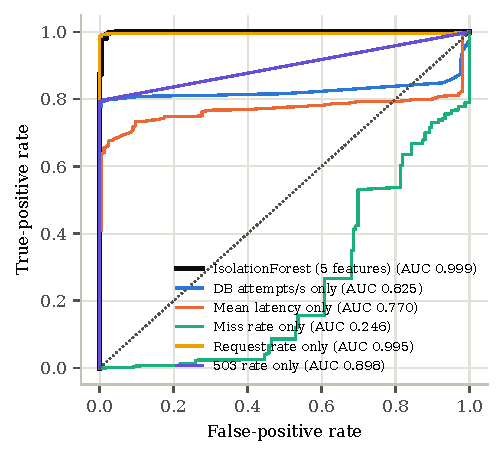
\includegraphics[width=0.56\linewidth]{figures/fig_roc.pdf}
\caption{ROC curves on held-out normal and attack intervals for the offline
IsolationForest and for each of its input features used alone as a score.}
\label{fig:roc}
\end{figure}

\begin{table}[t]
\centering
\caption{Offline IsolationForest: effect of the contamination parameter and of the
training-window size (test: 166 normal, 733 attack intervals).}
\label{tab:contam}
\small
\begin{tabular}{@{}lrrrr@{\hspace{2.2em}}lrrr@{}}
\toprule
\multicolumn{5}{@{}c}{Contamination (train $n=166$)} & \multicolumn{4}{c@{}}{Training size (contam.\ 0.01)} \\
\cmidrule(r{2.2em}){1-5}\cmidrule(l){6-9}
Value & Precision & Recall & FPR & AUC & $n$ & Recall & FPR & F1 \\
\midrule
0.01 & 0.996 & 0.989 & 0.018 & 0.999 & 10 & 0.156 & 0.012 & 0.269 \\
0.03 & 0.975 & 1.000 & 0.115 & 0.999 & 20 & 0.903 & 0.024 & 0.946 \\
0.05 & 0.959 & 1.000 & 0.187 & 0.999 & 50 & 0.874 & 0.042 & 0.928 \\
0.10 & 0.943 & 1.000 & 0.265 & 0.999 & 100 & 0.218 & 0.000 & 0.358 \\
     &       &       &       &       & 166 & 0.989 & 0.018 & 0.992 \\
\bottomrule
\end{tabular}
\end{table}

The training-size sweep reveals the detector's main fragility. With the first 10
normal intervals---the deployed minimum---recall on the held-out attack set is only
0.16; with 20 it is 0.90; but with 100 it falls back to 0.22 before recovering to 0.99
with all 166. The forest's decision threshold is set from the training scores, so its
operating point depends on which particular normal intervals happen to be in the
window (for example, whether a brief high-latency normal interval is present). This
non-monotonic behavior explains the one ``ready but silent'' ML miss in
Table~\ref{tab:episodes}, and argues for a longer minimum training window and for
fixing the decision threshold on a validation set rather than through
\texttt{contamination} alone.

\paragraph{Summary for RQ3.} The two detectors are complementary rather than
interchangeable. The IsolationForest is fast (sub-second median), dense (recall 0.91),
and adaptive, but depends on a clean, sufficiently long training window and flags any
departure from what it has seen, including idleness. The rule is slower and sparser
but perfectly precise, interpretable, available from the first second, and---because
it measures harm rather than novelty---silent on both absorbed bursts and defended
attacks. Together they detected every attack with one false alarm.

\subsection{End-to-End Validation}
\label{sec:validation}
The automated suite \texttt{tests/test\_cachecollapse.py} drives the live stack through
the same control API as the dashboard and samples the SSE feed. Its final run passed
all 16 cases (Table~\ref{tab:tests}). Its quantitative evidence---for example a peak of
227 DB q/s and 145 failures per interval under attack versus 11 q/s and none with
protection, and 20 of 20 storefront requests succeeding during a defended
attack---agrees with the log analysis above.

\begin{table}[t]
\centering
\caption{End-to-end test suite (final run: 16/16 passed).}
\label{tab:tests}
\small
\begin{tabularx}{\linewidth}{@{}rL{6.0cm}Y@{}}
\toprule
\# & Test & Evidence recorded \\
\midrule
1 & All 9 containers running & 9 up \\
2 & Dashboard page loads & HTTP 200, correct title \\
3 & Storefront loads & HTTP 200, ``CacheShop'' present \\
4 & Product API returns data & \texttt{/api/products/1} $\rightarrow$ 200 with name and price \\
5 & Cache works (second call faster) & 137 ms (DB) $\rightarrow$ 9 ms (cache) \\
6 & Unknown product returns 404 & \texttt{/api/products/99999} $\rightarrow$ 404 \\
7 & Baseline is calm & Peak DB 17 q/s; 0 alerts \\
8 & Attack overloads the DB & Peak latency 500 ms, DB 227 q/s, 145 failures per interval \\
9 & Rule detector fires on attack & 10 samples alerted \\
10 & ML detector fires on attack & 28 samples alerted \\
11 & Cache locking keeps DB load low & Peak DB 11 q/s (vs.\ 227 undefended) \\
12 & Protection preserves availability & Peak latency 152 ms, 0 failures \\
13 & System recovers after attack stops & Healthy again in ${\approx}2$ s \\
14 & Live feed updates faster than 1 s & Two samples 0.6 s apart differ \\
15 & Control endpoints respond & traffic / attack / defense / reset OK \\
16 & Storefront served while protected & 20/20 product requests succeed under attack + defense \\
\bottomrule
\end{tabularx}
\end{table}

%% =====================================================================
\section{Comparative Analysis}
\label{sec:comparative}
%% =====================================================================

\subsection{Capability Coverage}
CacheCollapse integrates concerns that prior work addresses only in prt
(Table~\ref{tab:capability}). Performance-oriented stampede work
\cite{vattani2015,nishtala2013} contributes coalescing and early recomputation but no
attacker model, detection, or testbed. Application-layer DDoS work
\cite{praseed2019,xie2009,ranjan2009} contributes detection and scheduling but neither
the cache-specific mechanism nor a reproducible container environment. Work on
cache- and CDN-targeting attacks \cite{nguyen2019,guo2020,triukose2009} demonstrates
attacks on shared edge caches but does not address the application-internal cache or
layered mitigation. Container-security work \cite{combe2016,sultan2019} catalogs
weaknesses without instrumenting a specific availability attack end to end. The Yo-Yo
attack \cite{sides2016,bremlerbarr2017} is closest in spirit but targets elasticity
rather than caching. Overload-control work \cite{welsh2001,welsh2003} supplies general
mechanisms without an attack model.

\begin{table}[t]
\centering
\caption{Capability coverage. \yes~= addressed; \prt~= partial; \no~= not addressed.
``Analytical'' denotes a quantitative model of the attack or its mitigation.}
\label{tab:capability}
\small
\begin{tabular}{@{}lcccccc@{}}
\toprule
Work & Adversarial & Testbed & Analytical & Detection & Layered mit. & Containerized \\
\midrule
Probabilistic prevention \cite{vattani2015} & \no & \no & \yes & \no & \prt & \no \\
Memcache leases \cite{nishtala2013} & \no & \no & \no & \no & \prt & \no \\
App-layer DDoS \cite{xie2009,praseed2019} & \yes & \no & \prt & \yes & \no & \no \\
DDoS-Shield \cite{ranjan2009} & \yes & \prt & \yes & \yes & \prt & \no \\
Flash crowds \cite{jung2002,kandula2005} & \yes & \prt & \no & \yes & \prt & \no \\
DDoS surveys \cite{mirkovic2004,zargar2013} & \yes & \no & \no & \prt & \prt & \no \\
CPDoS / CDN abuse \cite{nguyen2019,guo2020} & \yes & \yes & \no & \no & \prt & \no \\
Container security \cite{combe2016,sultan2019} & \prt & \no & \no & \no & \no & \prt \\
Yo-Yo attack \cite{sides2016,bremlerbarr2017} & \yes & \prt & \yes & \prt & \no & \yes \\
Overload control \cite{welsh2001,welsh2003} & \no & \yes & \prt & \prt & \prt & \no \\
\textbf{CacheCollapse} & \yes & \yes & \yes & \yes & \yes & \yes \\
\bottomrule
\end{tabular}
\end{table}

\subsection{Comparison of Mitigation Techniques}
Table~\ref{tab:mitigations} compares the mitigations available against a cache stampede
along six dimensions. Two observations stand out. First, the techniques fall into two
groups: those that reduce the \emph{probability} of a synchronized miss (TTL jitter,
early recomputation, longer TTLs) and those that bound its \emph{cost} once it happens
(single-flight, stale serving, rate limiting, admission control). An adversary who
can time bursts defeats the first group---jitter adds noise the attacker can average
away by probing, and early recomputation only refreshes keys that are being read
anyway---so a security-oriented design must include the second group. Second, within
the second group only edge-level controls protect the proxy and connection path. This
is the empirical result of Section~\ref{sec:ablation} restated as a design rule.

\begin{table}[t]
\centering
\caption{Comparison of stampede mitigations. ``Root cause'' = removes redundant
regeneration; ``Proxy'' = protects the proxy/connection path; ``Adversarial'' = remains
effective when bursts are deliberately timed.}
\label{tab:mitigations}
\footnotesize
\begin{tabularx}{\linewidth}{@{}L{3.1cm}cccccY@{}}
\toprule
Technique & Root cause & Protects DB & Proxy & Adversarial & Staleness & Cost / caveat \\
\midrule
Longer TTL & \no & \prt & \no & \no & Higher & Fewer but equally large stampedes (Eq.~\ref{eq:stampede}) \\
TTL jitter & \no & \prt & \no & \no & Same & De-synchronizes bulk fills only \\
Early recomputation (XFetch) \cite{vattani2015} & \prt & \prt & \no & \prt & Same & Needs regeneration-cost estimate; read-triggered \\
Single-flight lock / lease \cite{nishtala2013,singleflight} & \yes & \yes & \no & \yes & Same & Losers must wait or be served something \\
Stale-while-revalidate \cite{rfc5861} & \prt & \yes & \no & \yes & Bounded & Requires a stale copy (pre-warm) \\
App-layer rate limit & \no & \prt & \no & \prt & None & Acts after the proxy and app have paid for the request \\
Edge rate limit \cite{nginxlimitreq} & \no & \prt & \yes & \yes & None & Per-address; weak against many sources \\
Admission control \cite{welsh2003,cherkasova2002} & \no & \yes & \prt & \yes & None & Needs a load signal; may reject legitimate users \\
Auto-scaling & \no & \prt & \prt & \no & None & Slow; itself attackable (Yo-Yo) \cite{sides2016} \\
\textbf{CacheCollapse (lock + SWR + app + edge RL)} & \yes & \yes & \yes & \yes & Bounded (60 s) & Per-address limit; see Sec.~\ref{sec:limitations} \\
\bottomrule
\end{tabularx}
\end{table}

\subsection{Comparison of Detection Approaches}
Table~\ref{tab:detcompare} positions the two CacheCollapse detectors relative to
generic approaches. The comparison underlines why we chose to deploy both: a
volume threshold is cheap but cannot tell harm from popularity
(Table~\ref{tab:single}); behavioral models of browsing \cite{xie2009} and
session-suspicion scoring \cite{ranjan2009} require per-client modeling that a
stampede, made of identical requests for public objects, does not reward; supervised
classifiers require labelled attacks that rarely exist in production. The rule and
the unsupervised forest need neither per-client state nor labels.

\begin{table}[t]
\centering
\caption{Detection approaches for the cache-stampede IDDoS.}
\label{tab:detcompare}
\footnotesize
\begin{tabularx}{\linewidth}{@{}L{3.2cm}L{1.7cm}L{1.8cm}L{1.8cm}Y@{}}
\toprule
Approach & Labels needed & Detects harm or novelty & Explainable & Main weakness here \\
\midrule
Request-volume threshold & No & Novelty (volume) & Yes & Fires on absorbed bursts (97\%) \\
Per-client browsing model \cite{xie2009} & Normal only & Novelty & Partly & Stampede requests are individually normal \\
Session suspicion scoring \cite{ranjan2009} & No & Novelty & Partly & Many sources defeat per-session state \\
Supervised classifier & Attack + normal & Either & Rarely & Labelled attacks unavailable \\
\textbf{Multi-signal rule (ours)} & No & Harm & Fully & Conservative thresholds; recall 0.27 \\
\textbf{IsolationForest (ours)} & Normal only & Novelty & Weakly & Needs clean window; flags idleness \\
\textbf{Rule OR forest (ours)} & Normal only & Both & Partly & 12/12 episodes, FPR 0.3\% \\
\bottomrule
\end{tabularx}
\end{table}

\subsection{Positioning}
In summary, CacheCollapse is not a new mitigation primitive: single-flight
regeneration, stale serving, and rate limiting all predate it. Its contribution is to
treat the stampede as an adversarial availability problem and to show,
quantitatively and reproducibly, how these primitives must be composed, what each one
protects, how quickly they act, and how the attack can be detected without labels and
without confusing harm with popularity.

%% =====================================================================
\section{Discussion}
\label{sec:discussion}
%% =====================================================================

\subsection{Why a Layered Defense Is Necessary}
No single control is sufficient. Cache locking is the only mechanism that addresses the
root cause---it restores the $N{:}1$ query ratio to $1{:}1$, as the coalescing ratio of
4.7 shows---but it operates below the proxy and cannot relieve congestion of the
connection path. Stale-while-revalidate makes locking \emph{fast} by giving losers an
immediate answer, but only if a stale copy exists, which is why pre-warming matters.
Application-layer rate limiting sheds database work but acts too late: by the time the
application rejects a request, the proxy and the application have already paid for
it. Edge rate limiting protects the proxy but, on its own, would not fix the
redundant-query amplification of whatever traffic it admits. The correct design
composes them in the order requests encounter them: the edge limiter caps the flood,
cache locking coalesces the surviving misses, and stale-while-revalidate serves the
coalesced waiters without delay. This mirrors the prevention--detection--response
framing urged for DDoS defense \cite{zargar2013} and the overload-control principle of
shedding load as early as possible \cite{welsh2001,beyer2016}.

\subsection{Detecting Harm versus Detecting Novelty}
The detection results argue against treating the two detectors as substitutes, and
they suggest a sharper way to describe the difference than ``rules versus machine
learning''. The rule is a detector of \emph{harm}: it fires only when the database is
demonstrably overloaded, so it is silent on absorbed bursts, silent on defended
attacks, and silent when idle. The IsolationForest is a detector of \emph{novelty}: it
fires whenever the traffic vector leaves the region it was trained on, which happens
during attacks, but also during idleness and partly during defended attacks. Both
questions are useful. Harm is what an on-call engineer must act on; novelty is what a
security analyst wants to know about even when the defenses are holding, because a
defended attack is still an attack. A practical deployment should therefore route the
two signals differently---the rule to paging, the forest to a security dashboard---and
should give the forest an explicit notion of ``no traffic'' (for example, by not
scoring intervals with fewer than a minimum number of requests) to avoid the
closed-world false alarms we observed \cite{sommer2010}.

The analysis also shows that a plausible-sounding signal can be misleading. The
stampede narrative suggests that the cache-miss ratio should spike during an attack,
and it was included in the rule for that reason. In this testbed it does not: the short
TTL and uniform catalog make the normal miss ratio high (0.62), and during the attack
the high-volume, repeatedly requested hot keys are hits most of the time between
expiries, so the ratio actually falls (0.51). Equation~\eqref{eq:baseline} predicts the
first effect from first principles. The lesson for practitioners is to validate every
detection feature against a model or a measurement of normal behavior, and to prefer
signals that directly measure the protected resource (database attempts, pool
exhaustion) over proxies for it.

\subsection{Engineering Lessons from Building the Testbed}
\label{sec:lessons}
Several of the most instructive results emerged as bugs during development. Table
\ref{tab:bugs} summarizes them; each is a reusable lesson for anyone building or
defending a cached service.

\begin{table}[t]
\centering
\caption{Defects found during development, their causes, and the general lesson.}
\label{tab:bugs}
\footnotesize
\begin{tabularx}{\linewidth}{@{}L{2.9cm}L{3.3cm}L{3.3cm}Y@{}}
\toprule
Symptom & Root cause & Fix & General lesson \\
\midrule
Defended shop still slow; attacker throttled legitimate users & Limiter keyed on the proxy's address; all clients shared one budget & Proxy overwrites \texttt{X-Forwarded-For} with the real peer address & Per-client limits behind a proxy need trusted client identity \\
Defended latency up to ${\approx}2.5$~s & Lock losers queued behind the winner & Serve the stale copy immediately (SWR); pre-warm stale cache & Coalescing must not turn into queueing \\
Shop slow (300--700~ms) even with DB protected & Flood still congested Nginx and the app's threads & Edge \texttt{limit\_req}, toggled live via include + reload & Protect the request path, not only the database \\
Single false alarm at start of baseline & Cold cache: every request misses, looks like a stampede & Suppress alerts for 3~s warm-up; train ML only after it & Distinguish start-up transients from attacks \\
ML stopped recognizing attacks & Cold-start spike polluted the ``normal'' training set & Skip warm-up; standardize features & Training data hygiene determines unsupervised accuracy \\
Occasional one-interval ML alert & Noise in a single sample & Two-interval debounce; contamination 0.03$\rightarrow$0.01 & Debounce novelty detectors \\
Metric totals split and inconsistent & Several Gunicorn workers, each with its own counters & One worker, 200 threads & In-process metrics need a single process (or multiprocess mode) \\
Shop stuck ``red'' after attack ended & Browser fetches without timeout piled up & 4~s \texttt{AbortController} timeout; non-overlapping refresh & Clients need timeouts too, or they amplify outages \\
Dashboard felt laggy & 1~Hz sampling & 2~Hz sampling and streaming & Rates need enough samples per window; 2~Hz suffices \\
\bottomrule
\end{tabularx}
\end{table}

\subsection{Deployment Guidance}
For operators of cached, containerized web services, the results translate into the
following checklist:
\begin{enumerate}[leftmargin=*]
\item \textbf{Coalesce regeneration of hot keys} with a single-flight lock or lease,
and release locks with a token check \cite{kleppmann2016}.
\item \textbf{Keep a stale copy} of hot entries and serve it to lock losers
(stale-while-revalidate); pre-warm it at start-up so the defense works from the first
miss.
\item \textbf{Rate-limit at the edge}, not only in the application, and return 429
rather than 503 for intentional shedding (\texttt{limit\_req\_status 429}).
\item \textbf{Forward trusted client identity} from the proxy (overwrite, never
append, \texttt{X-Forwarded-For} at the outermost trusted hop) so per-client limits are
meaningful.
\item \textbf{Choose pool behavior deliberately.} A fail-fast pool converts overload
into immediate errors (good for shedding, bad for goodput under stampede); a bounded
wait with a short timeout may preserve more useful work.
\item \textbf{Monitor the protected resource directly}: database attempts, pool
exhaustion, and failures, together with latency. Validate any proxy signal (such as
miss ratio) against normal behavior before alerting on it.
\item \textbf{Run both a harm detector and a novelty detector}, route them to
different audiences, and train the novelty detector on a clean, sufficiently long
window that excludes start-up and idle periods.
\item \textbf{Treat TTLs as public.} Hit/miss timing reveals them; do not rely on
obscurity or jitter for protection.
\end{enumerate}
All of these are realizable with standard components---Redis, Nginx, and a metrics
pipeline---and none requires changes to application semantics beyond accepting bounded
staleness.

\subsection{Security of the Testbed and Ethical Considerations}
\label{sec:ethics}
CacheCollapse is a tool for generating denial-of-service traffic, and it was designed
to be safe by construction. The attack generator targets only the stack's own proxy on
a private network; no external system is ever contacted; and all data are synthetic.
The control API that launches attacks is intentionally unauthenticated for classroom
use, and Grafana ships with default credentials and anonymous viewing. These choices
are acceptable on a laptop but not on any reachable host. The project's deployment
plan accordingly restricts exposure to known addresses via a cloud firewall, requires
changing default passwords, and recommends local demonstration as the safest option;
a helper script that publishes the dashboard through a temporary tunnel should be used
only for short, supervised sessions, since anyone with the link can launch the attack
against the demo itself. The techniques described here are well known to defenders and
attackers alike; we believe that publishing a reproducible, defensive-first account of
them, with mitigations and detection, benefits defenders more than it helps attackers.

\subsection{Threats to Validity}
\label{sec:validity}
\paragraph{Construct validity (are we measuring what we claim?).} The log analysis
exposed several measurement subtleties that affect interpretation:
\begin{itemize}[leftmargin=*]
\item \emph{Database ``queries'' are attempts.} The counter is incremented before a
pool connection is obtained, so under overload it includes attempts rejected with 503.
We therefore report ``attempts'' and derive completed queries separately
(Section~\ref{sec:mechanics}).
\item \emph{Failures are logged as per-interval counts}, not per-second rates. With
0.5~s intervals the two differ by a factor of two; all rates in this paper divide by
the measured interval.
\item \emph{Hits and misses overlap under defense}, because a lock loser served stale
data is counted as both a miss and a hit; the defended miss ratio is therefore biased
low, while the coalescing ratio is unaffected.
\item \emph{Latency is measured inside the application.} It excludes time spent in the
proxy and requests rejected at the edge; the storefront and the test suite provide the
complementary end-to-end view.
\item \emph{p95 latency is quantized} to histogram bucket bounds and is therefore
reported only as supporting evidence.
\item \emph{Edge rejections are invisible to the application metrics} and, with Nginx
defaults, are HTTP~503 at the client.
\item \emph{Per-container CPU and memory} were part of the original specification but
are not collected by the final monitor (Prometheus scrapes only the application), so
no resource-utilization results are reported.
\item \emph{Defense configuration is not logged per interval.} The mode ``protected''
means ``at least one defense on''; the ablation therefore relies partly on observation
and on the session history rather than on per-interval labels.
\end{itemize}

\paragraph{Internal validity.} The attacker, the victim, and the monitor share one
host's CPU, so heavy attack traffic also slows the instrumentation; the monitor's
sampling interval stretches under load (median 0.53~s overall, longer during attacks).
Mode labels can lag traffic changes by up to one interval, which affects detection
latencies at the 0.5~s scale but not episode-level conclusions.

\paragraph{External validity.} The testbed is a single-host Docker Desktop deployment
whose port forwarding adds latency under heavy connection load, so absolute latencies
are environment-specific while relative effects are robust. Traffic is synthetic:
popularity is uniform rather than Zipf-like \cite{breslau1999}, database cost is
modelled with \texttt{pg\_sleep}, and both normal and attack traffic originate from a
single load-generator address. The last point has two consequences: the edge limiter
also throttles the synthetic normal traffic (which is why defended database load falls
below the baseline), and per-address limiting is easier than it would be against a
distributed attacker using many addresses. Legitimate-user availability under defense
is therefore evidenced by the storefront and test case~16, which originate from a
different address, rather than by the synthetic background traffic.

\paragraph{Conclusion validity.} The main results come from one final session.
Consecutive intervals are autocorrelated, so bootstrap intervals computed over
intervals understate uncertainty; the episode-level and cross-session results
(Figures~\ref{fig:dev} and~\ref{fig:detlat}) provide the more conservative evidence and
are consistent with the interval-level estimates.

\subsection{Limitations}
\label{sec:limitations}
Beyond the validity threats above, the study has the following limitations. The
IsolationForest requires a clean baseline window, so a system attacked from start-up
trains on contaminated data or not at all (as in the first episode of the final
session); the always-available rule mitigates but does not eliminate this. Thresholds
($K$, $\tau_L$, $\tau_m$, limiter rates) were tuned on the testbed and need site-specific
calibration. The edge limiter is per source address and would need to be complemented
by aggregate or behavioral limiting against a widely distributed attacker. Finally, the
study evaluates a single cache, a single database, and a single application replica;
interactions with replication, sharding, and auto-scaling are left to future work.

%% =====================================================================
\section{Conclusion and Future Work}
\label{sec:conclusion}
%% =====================================================================

CacheCollapse is a reproducible containerized framework for studying and defending
the cache-stampede indirect denial of service---an availability attack in which
well-formed requests, aligned with cache expiry, overload a database through the
application rather than by attacking it directly. We revisit the four research
questions.

\textbf{RQ1 (Reproduction).} On a nine-container Nginx--Flask--Redis--PostgreSQL stack,
an attacker rotating 250-request bursts across 20 hot products raised the median rate
of database query attempts from 11 to 108 per second (peak 317), more than doubled
median latency (77 to 174~ms, peak 1.16~s), and produced HTTP~503 failures in 80\% of
sampling intervals, at a median of 84 failures per second.

\textbf{RQ2 (Mechanism).} A simple model predicts the baseline database load to within
9\% from the catalog size, TTL, and request rate, and explains why the normal miss
ratio is already high under short TTLs. Under attack, a fail-fast connection pool and
failed regenerations that never fill the cache combine into goodput collapse:
completed database work stays near 23 queries per second---about one fifth of the
pool's nominal capacity---while every additional attempt fails.

\textbf{RQ3 (Detection).} The multi-signal rule detected 11 of 12 attack episodes with
perfect precision and a median latency of 3.2~s; the IsolationForest detected 10 of 12
with a median latency of 0.85~s and interval recall of 0.91. Their union detected all
12 with a single false alarm in 332 normal intervals. The rule detects harm and is
silent on high-volume traffic that the cache absorbs (where a volume threshold fires
97\% of the time); the forest detects novelty, which makes it fast but also makes it
flag idleness. Threshold analysis shows the deployed rule is conservative and could
roughly double its recall at a small false-alarm cost, and that its cache-miss
condition is a weak signal that should be replaced by direct measures of database
harm.

\textbf{RQ4 (Mitigation).} Cache locking with stale-while-revalidate plus application
and edge rate limiting reduced median database load 18-fold (95\% CI 16.8--19.2) to
6 queries per second, cut median latency 6.4-fold to 27~ms, effectively eliminated
failures, held for 4.5~hours of continuous attack, and restored health a median of
1.35~s after being enabled mid-attack. The ablation and the longitudinal analysis of
14 sessions establish that database-level coalescing and edge-level rate limiting
protect different parts of the system and are both required.

\paragraph{Future work.} Several directions follow naturally. (1)~\emph{Realistic
workloads}: replay production-like traces with Zipf-distributed popularity and
measure how skew changes both the stampede and the miss-ratio signal. (2)~\emph{Distributed
attackers}: generate attack traffic from many addresses and evaluate aggregate,
behavioral, and adaptive admission control \cite{welsh2003,ranjan2009} in place of
per-address limits. (3)~\emph{Orchestrated deployments}: extend the testbed to
multi-node Kubernetes with replicated caches and auto-scaling, to study interactions
with Yo-Yo-style attacks \cite{sides2016,bremlerbarr2017}. (4)~\emph{Proactive
mitigation}: add probabilistic early recomputation \cite{vattani2015} and token-checked
leases \cite{kleppmann2016} and compare them with the current reactive locking.
(5)~\emph{Better detection}: replace the miss-ratio condition with pool-exhaustion and
failure signals, calibrate thresholds automatically from a validation window, give the
forest an explicit no-traffic state, and log the active defense configuration with
every sample. (6)~\emph{Instrumentation}: add per-container resource metrics (for
example via cAdvisor) and end-to-end latency measured at the proxy.

%% =====================================================================
%% Back matter (Elsevier-style declarations)
%% =====================================================================

\section*{CRediT Authorship Contribution Statement}
\textbf{Manal Aamir:} Conceptualization, Methodology, Writing -- Review and Editing.
\textbf{Tayyaba Arshad:} Investigation, Validation, Data Curation.
\textbf{Noor Afza:} Software (load generation and monitoring), Visualization.
\textbf{Batool Fatima:} Software (detection and mitigation), Validation.
\textbf{Aun Zaidi:} Conceptualization, Methodology, Software (system integration),
Writing -- Original Draft.

\section*{Declaration of Competing Interest}
The authors declare that they have no known competing financial interests or personal
relationships that could have appeared to influence the work reported in this paper.

\section*{Funding}
This work was carried out as the Complex Engineering Problem of course SE-401
Information Security, Spring 2026, at NED University of Engineering and Technology. It
received no specific grant from any funding agency in the public, commercial, or
not-for-profit sectors.

\section*{Data and Code Availability}
All source code (Docker Compose definition, application, load generator, monitor,
detectors, dashboards, and test suite) and the 18 monitoring logs analyzed in this paper
are held in the project repository and are available from the authors on request. The
repository contains no real user data; all product records are synthetic.

%% NOTE TO AUTHORS: Elsevier journals require this declaration when generative AI
%% tools were used in preparing the manuscript. Edit it to describe your actual use,
%% or delete it if it does not apply.
\section*{Declaration of Generative AI and AI-Assisted Technologies in the Writing Process}
During the preparation of this work the authors used AI-assisted tools to help analyze
the experiment logs, generate figures, and draft and edit parts of the text. After
using these tools, the authors reviewed and edited the content as needed and take full
responsibility for the content of the publication.

\section*{Acknowledgments}
The authors thank the course instructor of SE-401 Information Security for guidance on
the scope of the Complex Engineering Problem.


\bibliographystyle{elsarticle-num}
\bibliography{references}

\clearpage
\appendix
%% =====================================================================
%% Appendices
%% =====================================================================

\section{Reproduction Guide}
\label{app:repro}

\paragraph{Prerequisites.} Docker Desktop (or Docker Engine with the Compose plugin),
about 2~GB of free RAM, and a free TCP port 8090 (configurable as \texttt{PUBLIC\_PORT}
in \texttt{.env}). Python~3 is needed only to run the test suite.

\paragraph{Start the stack.}
\begin{lstlisting}[language=bash, numbers=none]
docker compose up --build        # first run downloads images and builds (minutes)
docker compose ps                # all 9 services Up; db (healthy)
\end{lstlisting}

\paragraph{Endpoints.}
\begin{center}
\small
\begin{tabular}{@{}ll@{}}
\toprule
Dashboard (live operations console) & \url{http://localhost:8090} \\
CacheShop storefront & \url{http://localhost:8090/shop.html} \\
Product API & \url{http://localhost:8090/api/products/<id>} \\
Grafana & \url{http://localhost:3000} \\
Prometheus & \url{http://localhost:9090} \\
\bottomrule
\end{tabular}
\end{center}

\paragraph{Run the three experiments.} Use the dashboard presets \emph{Exp~1}
(baseline), \emph{Exp~2} (attack, no defense), and \emph{Exp~3} (attack with defenses),
or call the control API directly:
\begin{lstlisting}[language=bash, numbers=none]
curl -X POST localhost:8090/control/preset -H 'Content-Type: application/json' -d '{"exp":1}'
curl -X POST localhost:8090/control/preset -H 'Content-Type: application/json' -d '{"exp":2}'
curl -X POST localhost:8090/control/reset
curl -X POST localhost:8090/control/preset -H 'Content-Type: application/json' -d '{"exp":3}'
\end{lstlisting}
Allow at least 5--10~s of baseline traffic before an attack so that the ML detector can
train. Each monitor start creates a new \texttt{results/metrics\_<timestamp>.csv}.

\paragraph{Validate.}
\begin{lstlisting}[language=bash, numbers=none]
python tests/test_cachecollapse.py   # expected: SUMMARY: 16 passed, 0 failed
\end{lstlisting}

\paragraph{Stop.} \texttt{docker compose down} (add \texttt{-v} to remove volumes).

\section{Key Configuration Listings}
\label{app:listings}

\begin{lstlisting}[caption={Nginx: edge rate-limit zone, client-address forwarding, and the live-reloadable include (excerpt of \texttt{nginx/nginx.conf}).}, label={lst:nginx}]
limit_req_zone $binary_remote_addr zone=api_rl:10m rate=50r/s;
upstream backend { server backend:5000; keepalive 64; }

location /api/ {
    proxy_set_header X-Forwarded-For $remote_addr;   # overwrite, not append
    proxy_set_header X-Real-IP $remote_addr;
    include /etc/nginx/dynamic/ratelimit.conf;      # rewritten by the monitor
    proxy_http_version 1.1;
    proxy_set_header Connection "";
    proxy_pass http://backend/;
}
# dynamic/ratelimit.conf when ON:
#   limit_req zone=api_rl burst=20 nodelay;
\end{lstlisting}

\begin{lstlisting}[caption={Nginx container command: start Nginx and reload it whenever the edge rate-limit include changes (excerpt of \texttt{docker-compose.yml}).}, label={lst:watcher}]
nginx -g 'daemon off;' &
prev=""
while :; do
  sleep 1
  cur=$(cat /etc/nginx/dynamic/ratelimit.conf 2>/dev/null)
  if [ "$cur" != "$prev" ]; then prev="$cur"; nginx -s reload 2>/dev/null; fi
done
\end{lstlisting}

\begin{lstlisting}[language=Python, caption={Rule-based detector (\texttt{monitor/detect\_rules.py}).}, label={lst:rule}]
DB_MULTIPLIER = 5       # "high DB load" = more than 5x the learned baseline
BASELINE_FLOOR = 5      # never treat less than this many q/s as the baseline
RESP_MS_LIMIT = 200     # "high response time"
MISS_RATE_LIMIT = 0.5   # "high miss rate"

def evaluate(sample, baseline_db):
    base = max(baseline_db, BASELINE_FLOOR)
    c1 = sample["db_qps"] > DB_MULTIPLIER * base
    c2 = sample["resp_avg_ms"] > RESP_MS_LIMIT
    c3 = sample["miss_rate"] > MISS_RATE_LIMIT
    return {"db_load": c1, "response": c2, "miss_rate": c3}, (c1 and c2 and c3)
\end{lstlisting}

\begin{lstlisting}[language=Python, caption={IsolationForest detector core (\texttt{monitor/detect\_ml.py}).}, label={lst:ml}]
FEATURES = ["db_qps", "resp_avg_ms", "miss_rate", "rps", "failed"]
MIN_TRAIN = 10

def observe_baseline(self, sample):
    self._baseline.append([sample[f] for f in FEATURES])
    if len(self._baseline) >= MIN_TRAIN:
        self._baseline = self._baseline[-300:]
        data = np.array(self._baseline, dtype=float)
        self._scaler = StandardScaler().fit(data)
        self._model = IsolationForest(contamination=0.01, random_state=0)
        self._model.fit(self._scaler.transform(data))

def score(self, sample):
    if self._model is None:
        return 0.08, False
    x = self._scaler.transform([[sample[f] for f in FEATURES]])
    raw = float(self._model.decision_function(x)[0])  # +normal / -anomaly
    return max(0.0, min(1.0, 0.5 - raw * 4.0)), self._model.predict(x)[0] == -1
\end{lstlisting}

\section{Mapping to the Attributes of a Complex Engineering Problem}
\label{app:cep}
Table~\ref{tab:cep} maps the project onto the attributes of a complex engineering
problem defined in the International Engineering Alliance's graduate attributes
\cite{ieagapc2021}, which underlie the accreditation criteria applied to this course.

\begin{table}[h]
\centering
\caption{Complex engineering problem attributes addressed by CacheCollapse.}
\label{tab:cep}
\footnotesize
\begin{tabularx}{\linewidth}{@{}L{3.6cm}Y@{}}
\toprule
Attribute & How it is addressed \\
\midrule
WP1 Depth of knowledge & Caching theory, queueing and overload (Sec.~\ref{sec:bg-queueing}), rate-limiting algorithms, anomaly detection (Sec.~\ref{sec:bg-iforest}), container orchestration \\
WP2 Range of conflicting requirements & Database protection vs.\ user latency vs.\ data freshness vs.\ false alarms (tensions T1--T3, Sec.~\ref{sec:intro}) \\
WP3 Depth of analysis & Analytical model (Sec.~\ref{sec:model}), statistical evaluation, threshold sensitivity, ROC, ablation, longitudinal analysis (Sec.~\ref{sec:results}) \\
WP4 Familiarity of issues & Reframes a known performance hazard as an adversarial, emergent availability attack that cannot be patched \\
WP5 Extent of applicable codes & HTTP semantics (RFC 6585, RFC 5861), OWASP API Top 10, MITRE ATT\&CK, NIST SP 800-61 (Sec.~\ref{sec:threat}) \\
WP6 Stakeholder involvement & End users, operators, security analysts, instructor/audience; separate harm and novelty alerting for operators vs.\ analysts \\
WP7 Interdependence & Nine interacting services; defenses at different layers that are only effective in combination (Sec.~\ref{sec:ablation}) \\
\bottomrule
\end{tabularx}
\end{table}

\section{Glossary}
\label{app:glossary}
\begin{description}[leftmargin=1.2em,style=nextline,itemsep=1pt]
\item[Cache-aside] Pattern in which the application reads the cache and, on a miss,
loads from the database and fills the cache.
\item[Cache stampede (dog-pile, thundering herd)] Many concurrent misses for the same
key regenerating it simultaneously.
\item[Coalescing ratio $\rho$] Cache misses per database attempt; 1 without coalescing.
\item[Edge rate limiting] Limiting applied at the outermost proxy, before requests
consume upstream resources.
\item[Fail-fast pool] A connection pool that rejects requests immediately when all
connections are in use.
\item[Goodput] Useful completed work per unit time, as opposed to attempted work.
\item[IDDoS] Indirect (distributed) denial of service: overloading one component by
sending legitimate requests to another.
\item[IsolationForest] Unsupervised anomaly detector that scores points by how quickly
random trees isolate them.
\item[Single-flight] Allowing only one in-progress regeneration per key.
\item[Stale-while-revalidate (SWR)] Serving a slightly old copy while one request
refreshes the entry.
\item[TTL] Time-to-live of a cache entry.
\end{description}


\end{document}
